% !TeX spellcheck = de-DE

%--------------------------------------
%   Header
%--------------------------------------
\documentclass[
    appendixprefix=true,
    a4paper,                    % Papierformat A4
    10pt,                       % Schriftgröße 10pt
    %headings=normal,           % kleinere Überschriften verwenden
    chapterprefix=false,        % Einfügen von "Anhang" bzw. "Kapitel" in Überschrift
    oneside,                    % oneside - twoside
    openright,                  % einseitiges > Latex Workshop: Build with recipe
    titlepage,                  % Titleseite verwenden
    listof=totoc,               % alle Listen in das Inhaltsverzeichnis
    headsepline,                % Trennlinie zum Seitenkopf Bereich headings
    plainheadsepline,           % Trennlinie zum Seitenkopf Bereich Plain
    bibliography=totoc,         % das Literaturverzeichnis in den TOC
    parskip=half-,              % Abstand nach Absatz
    numbers=noenddot            % damit hinter der letzten Ziffer kein Punkt steht (Kapitelnummerierung)
]{scrreprt}

\newcommand{\art}{Bachelorarbeit}
\newcommand{\titel}{Design und Implementierung eines Web-basierten Analysetools für Bildungsportale}
\newcommand{\untertitel}{}
\newcommand{\autor}{Chris Dreyße}
\newcommand{\registriernr}{Nr. AI-2024-BA-051}
\newcommand{\hochschule}{Fachhochschule Erfurt}
\newcommand{\fachgebiet}{Angewandte Informatik}
\newcommand{\erstgutachter}{Prof. Marcel Spehr}
\newcommand{\zweitgutachter}{Herr Benedict Staack}
\newcommand{\datum}{28. März 2025} % \today gibt heutiges Datum aus, oder klassisch durch Abgabedatum zu ersetzen
\newcommand{\keywords}{aa,bb,cc,dd}
\newcommand{\ort}{Erfurt}	% persönlich Daten
%%--------------------------------------
%%   Packages
%%--------------------------------------

\usepackage[utf8]{inputenc}        	% Zeichenkodierung - !!!Achtung, alle Dateien auch im UTF8 speichern!!!
\usepackage[T1]{fontenc}            % westeuropäische Schriftzeichenkodierung
\usepackage[ngerman]{babel}        	% Babel-System - neue deutsche Rechtschreibung
\usepackage[left=4cm, right=3cm, top=2.5cm, bottom=2.5cm]{geometry} % Seitenränder



% Erlaubt sinnvolle URL-Umbrüche
\usepackage[hyphens]{url}
\usepackage{breakurl}
\usepackage{etoolbox}



% Literaturverzeichnis kompakter (aber mit etwas Abstand)
\apptocmd{\bibsetup}{\sloppy\clubpenalty4000\widowpenalty4000\relax}{}{}

% Optional: Etwas mehr Stretch für lange URLs
\setlength{\emergencystretch}{1.5em}


%---------------------------------------
%  Befehl für Schriftart Helvet / Arial
%---------------------------------------
\usepackage{helvet}						% Alternative Schriftart: lmodern
\renewcommand{\familydefault}{\sfdefault}	%serifenlos

\usepackage[onehalfspacing]{setspace}   % 1,5 facher Zeilenabastand aber nur im text nicht in Fußnoten oder Verzeichnissen

\usepackage{amssymb}        			% Mathesymbole
\usepackage{amsfonts}        			% mathematische Schriftarten
\usepackage{amsmath}       				% Mathepaket
\usepackage{cancel}            			% Durchstreichungen wie beim kürzen
\usepackage{mathcomp}        			% weitere Symbole
\usepackage{scrhack}        			% verbessert einige Fremdklassen in Zusammenspiel mit KomaScript
\usepackage[babel,german=quotes]{csquotes}	%Zitate
\usepackage[ngerman]{translator}		% Übersetzt Wörter die Latex setzt korrekt (wie z.B. "`Abbildung"')
%\usepackage{epstopdf}					
\usepackage{tikz}           		 	% Für selbsterstellte Graphiken
\usepackage{booktabs}        			% Für schönere Tabellen
\usepackage{array}                  	% erweiterte Tabelleneigenschaften
\usepackage{graphicx}               	% Grafiken
\usepackage{subfigure}              	% Grafiken nebeneinander mit (a) und (b)


\usepackage[hyphens]{url} % erlaubt Umbrüche in URLs
\usepackage{breakurl} 



%--------------------------------------
%   PDF Lesezeichen und Hyperlinks
%--------------------------------------
\usepackage[
pdfauthor={\autor},
pdftitle={{\titel { - }\untertitel}},
pdfsubject={{\titel { - }\untertitel}},
pdfkeywords={\keywords},
pdfpagelabels = {true},
pdfstartview = {FitV},
colorlinks = {true},
linkcolor = {black},
citecolor = {black},
urlcolor = {blue},
bookmarksopen = {true},
bookmarksopenlevel = {3},
bookmarksnumbered = {true},
plainpages = {false},
hypertexnames = {false}
]{hyperref}


%%--------------------------------------
%%   Glossar
%%--------------------------------------
%\usepackage[toc,acronym,nonumberlist]{glossaries}
%\makeglossaries




%--------------------------------------
%   Kopf- & Fußzeile 
%--------------------------------------
\usepackage[automark,plainheadsepline,autooneside]{scrlayer-scrpage}
\pagestyle{scrheadings}
\clearpairofpagestyles                                  % Kopf und Fußzeile löschen
\ihead[\hochschule]{\hochschule}                        % im Kopf -> links
\ohead[\fachgebiet]{\fachgebiet}                        % im Kopf -> rechts
\cfoot[\pagemark]{\pagemark}                            % Seitenzahl -cfoot für center - ofoot für outer
\renewcommand*{\headfont}{\upshape\sffamily\scriptsize} % Schrift Kopfzeile
\renewcommand*{\footfont}{\normalfont\sffamily\small}   % Schrift Fußzeile


%--------------------------------------
%   Quellcode-Listing Einstellungen
%   ftp://ftp.tu-chemnitz.de/pub/tex/macros/latex/contrib/listings/listings.pdf
%--------------------------------------

\usepackage{xcolor,listings}               	% bindet das Paket Listings ein
\definecolor{comment}{rgb}{.15,.4,.15}     	% hellgruen
\definecolor{keywd1}{rgb}{.15,.15,.6}      	% dunkelblau
\definecolor{keywd2}{rgb}{.35,.5,.55}      	% hellblau
\definecolor{string}{rgb}{.5,.15,.15}      	% dunkelrot
\definecolor{gray}{rgb}{0.4,0.4,0.4}		
\definecolor{darkblue}{rgb}{0.0,0.0,0.6}
\definecolor{cyan}{rgb}{0.0,0.6,0.6}


% Hier kann jetzt alles für die verwendete Sprache eingestellt werden
% Der lstset-Befehl ermöglicht haufenweise Einstellungen zur Formatierung

\lstset{language=C++,                            % hier Sprache einstellen
    basicstyle={\small} ,                        % Schriftgröße
    keywordstyle=\color{blue!80!black!100},      % Farbe der keywords
    identifierstyle=,                            % Bezeichnerstyle, hier leer
    commentstyle=\color{green!50!black!100},     % Farbe der Kommentare
    stringstyle=\ttfamily,                       % Aussehen der Strings
    breaklines=true,                             % Automatische Zeilenumbrüche
    numbers=left,                                % Zeilennummerierung links
    numberstyle=\small,                          % Größe der Zeilennummerierung
    frame=single,                                % einfacher Rahmen
    backgroundcolor=\color{blue!3},              % Hintergrundfarbe
    caption={Code},                              % Standardüberschrift
    captionpos=t,                                % Überschift oben (top)
    showspaces=false,							 % Leerzeichen nicht anzeigen
    showstringspaces=false,						 % Stringleerzeichen nicht anzeigen
% %UTF8 gebastle verdammtes tex grml
    literate= %
        {Ä}{{\"A}}1
        {Ö}{{\"O}}1
        {Ü}{{\"U}}1
        {ß}{{\ss}}1
        {ä}{{\"a}}1
        {ö}{{\"o}}1
        {ü}{{\"u}}1
        {~}{{\textasciitilde}}1
}

%\lstdefinelanguage{XML}
%{
%morestring=[b]",
%morestring=[s]{>}{<},
%morecomment=[s]{<?}{?>},
%stringstyle=\color{black},
%identifierstyle=\color{darkblue},
%keywordstyle=\color{cyan},
%morekeywords={xmlns,version,type}% list your attributes here
%}



%----------Worttrennung-----------
%---Latex trennt eigentlich recht gut, aber Fremdwörter o.ä. manchmal nicht, daher kann man Latex das Trennen einzelner Wörter beibringen, z.B.:
%\hyphenation{Ein-gangs-pro-zess}
%\hyphenation{Aus-gangs-pro-zess}
%\hyphenation{Web-client}
%\hyphenation{DMS-Web-client}
			% Pakete

\usepackage{listings}
\usepackage{xcolor}
\usepackage{tabularx}
\usepackage{xltabular}
\usepackage{float}
\usepackage{placeins}
\usepackage{longtable}
%--------------------------------------
%  Bitte den Editor auf Biblatex bzw. Biber einstellen!!! 
%--------------------------------------
\usepackage[style = alphabetic]{biblatex}			% Literaturverzeichnis, bei Style den Stil einstellen, vorzugsweise numeric oder alphabetic
\addbibresource{bib/literatur.bib}	% verwendete Literatur eintragen
%\newglossaryentry{latex}{
    name=latex,
    description={Danny Is a mark up language specially suited for scientific documents}
}

\newglossaryentry{maths}{
    name=mathematics,
    description={Mathematics is what mathematicians do}
}

\newglossaryentry{TestCode}{
    name={TestName2},
    description={TestBeschreibung3}
}		% Glossar


\lstdefinelanguage{Apache}{
    basicstyle=\ttfamily,
    sensitive=false,
    morekeywords={GET, POST, HTTP},
    morestring=[b]",
    morecomment=[l]{\#}
}

%--------------------------------------
%   Dokumentenbeginn
%--------------------------------------
\begin{document}
    \begin{titlepage}
    \pdfbookmark[-1]{\titel}{Marke}                    %Titel wird bei Lesezeichen angezeigt

    \titlehead{
        \begin{flushright}
            
\includegraphics[width=0.45\textwidth]{images/Logo_Informatik}
        \end{flushright}
    }
    \subject{\art \\ in der Angewandten Informatik\\ \large{\mdseries{\registriernr}}}     % Art der Arbeit
    \title{\Huge\titel}                                % Titel der Arbeit
    \subtitle{\Large\untertitel}                    % ggf. Untertitel
    \vspace{5em}
    \author{\textbf{\autor}}                            % Verfasser
    \date{Abgabedatum: \datum}                          % Datum
    \publishers{\erstgutachter \\ \zweitgutachter}        % Betreuer
    \maketitle
\end{titlepage}


% --- Ab hier in Römischen Zahlen nummerieren
    \pagenumbering{Roman}
    \pdfbookmark[0]{Kurzfassung}{MKurzfassung}
\begin{abstract}
    \section*{Kurzfassung}
    \label{sec:Kurzfassung}

    Diese Abschlussarbeit, welche im Rahmen eines Bachelorstudiums an der Fachhochschule Erfurt im Studiengang Angewandte Informatik angefertigt wurde, befasst sich mit dem Design und der Implementierung eines Web-basierten Analysetools zur Untersuchung des Nutzerverhaltens auf einem Bildungsportal. Ziel der Arbeit ist die Entwicklung einer datenschutzkonformen Lösung zur Erfassung, Auswertung und Visualisierung von Nutzungsdaten am Beispiel des Bildungsportals \textit{evaschiffmann.de}. 

    Im Mittelpunkt steht die Integration des Webanalyse-Tools Matomo sowie die Darstellung und Aufbereitung der erfassten Daten über das Dashboard-Tool Grafana. Dazu wurden geeignte Metriken und Key Performance Indicators definiert, welche eine gezielte Analyse der Nutzerinteraktionen ermöglichen. Ein wesentlicher Bestandteil der Analyse ist die Nachvollziehbarkeit einzelner Nutzersitzungen sowie der Auswertung von Interaktionen mit den zentralen Elementen der Website wie Tagebucheinträgen und Überschriften. 
    
    Die Implementierung erfolgte in einer containerisierten Umgebung mithilfe von Docker und Docker Compose, um eine einfache Reproduzierbarkeit und eine problemlose Bereitstellung im Live-Betrieb zu gewährleisten. Die entwickelte Anwendung wurde sowohl technisch als auch mittels einer Nutzerbefragung in Form eines Fragebogens evaluiert. Die Ergebnisse der Evaluation zeigen, dass die Lösung eine praktikable und übersichtliche Möglichkeit zur Analyse des Nutzerverhaltens darstellt.

    Die Arbeit richtet sich in erster Linie an die Anwender der Professur für Geschichtsdidaktik, welche die entwickelte Lösung im Rahmen ihrer Forschung nutzen werden. Darüber hinaus wendet sie sich an Bildungseinrichtungen und Privatpersonen, welche an der Erhebung und Visualisierung von Nutzerdaten im Bildungsbereich interessiert sind.

\end{abstract}

\pdfbookmark[0]{Abstract}{MAbstract}
\begin{abstract}
    \section*{Abstract}
    \label{sec:Abstract}
    This bachelor thesis, developed as part of a degree in Applied Computer Science at the University of Applied Sciences Erfurt, focuses on the design and implementation of a web-based analytics tool for examining user behavior on an educational platform. The aim of the thesis is to develop a solution for collecting, analyzing, and visualizing usage data for the educational website \textit{evaschiffmann.de}.

    At the core of the project is the integration of the web analytics tool Matomo, as well as the presentation and processing of the collected data using the dashboard tool Grafana. To support targeted analysis of user interactions, appropriate metrics and key performance indicators were defined. A key component of the analysis is the ability to track individual user sessions and evaluate interactions with central elements of the website, such as diary entries and collapsible headings.

    The implementation takes place within a containerized environment using Docker and Docker Compose to ensure reproducibility and facilitate future deployment in a live setting. The developed application was evaluated both technically and through a user survey in the form of a questionnaire. The evaluation confirmed that the tool proves to be a practical and effective solution for the structured analysis of user behavior.

    The thesis is primarily intended for the users at the Chair of History Didactics at the Friedrich Schiller University Jena, who will use the developed analytics tool in their research. Furthermore, it is aimed at educational institutions and private individuals interested in collecting and visualizing user data in the field of digital education.

\end{abstract}


%--------------------------------------
%   Inhalts-, Abbildungs-, Tabellenverzeichnis
%--------------------------------------
%\pdfbookmark[0]{\contentsname}{tocanc}
    \tableofcontents        % Inhaltsverzeichnung
    \listoffigures          % Abbildungsverzeichnis
    \listoftables           % Tabellenverzeichnis
    \lstlistoflistings      % Listingsverzeichnis
    \cleardoublepage        % sichert korrekte Seitenzahlen

%--------------------------------------
%   Zähler für römische Nummerierung speichern
%--------------------------------------
    \newcounter{exterior}                       % neuer Zähler (leer)
    \setcounter{exterior}{\value{page}}         % aktuelle Seitenzahl in neuen Zähler speichern

% --- Ab hier in Arabische Zahlen nummerieren
    \setcounter{page}{1}
    \pagenumbering{arabic}

% --- Hier ensprechend die Kapitel hinzufügen
    \chapter{Einleitung}
\label{ch:einleitung}

\section{Motivation}
\label{sec:motivation}

Die Nutzung von Online-Bildungsportalen hat sich in den letzten Jahren zu einem zentralen Bestandteil moderner Bildungsstrategien entwickelt und nimmt weiterhin stetig zu. Laut Eurostat nutzten im Jahr 2023 etwa 30 \% der Internetnutzer in der Europäischen Union im Alter von 16 bis 74 Jahren Online-Kurse oder digitale Lernmaterialien – ein Anstieg von 2 Prozentpunkten im Vergleich zum Vorjahr \parencite{Eurostat}. Aus einer Untersuchung der Potomac University geht des Weiteren hervor, dass 70 \% der Universitätsstudenten Online-Lernen als vorteilhafter im Vergleich zum traditionellen Unterricht bewerten \parencite{Potomac}. Diese Umfragen verdeutlichen, dass digitale Bildungsportale die Wissensvermittlung nachhaltig verändern und mittlerweile traditionelle Lehrmethoden ergänzen. Sie zeigen auf, wie wichtig digitale Angebote inzwischen geworden sind und welches Potenzial diese für die Wissensvermittlung haben.

Angesichts dieser Entwicklung stellt sich vor allem aus didaktischer, aber auch aus technischer Sicht die Frage, wie das Lernverhalten auf Bildungsportalen analysiert werden kann. Für die Professur für Geschichtsdidaktik der Friedrich-Schiller-Universität Jena, welche das Bildungsportal \textit{evaschiffmann.de} betreibt, gewinnt diese Fragestellung zunehmend an Bedeutung. Es ist von besonderem Interesse zu verstehen, wie Nutzer mit dem digitalisierten, historischen Wissen umgehen. Vor diesem Hintergrund soll eine Lösung geschaffen werden, welche die Professur bei der Untersuchung des Nutzerverhaltens unterstützt.

\section{Zielsetzung}
\label{sec:zielsetzung}

In einem gemeinsamen Gespräch mit Herrn Staack von der Professur für Geschichtsdidaktik wurden die Anforderungen an die Datenanalyse definiert. Dabei wurde besonderes Augenmerk auf die detaillierte Nachvollziehbarkeit einzelner Nutzersitzungen gelegt. Es soll möglich sein, zu analysieren, welche Seiten ein Nutzer aufruft und wie dieser mit den Elementen der Website interagiert. Besonders relevant sind die Interaktionen mit den Kernelementen des Bildungsportals – den Tagebucheinträgen und den interaktiven Überschriften. Zudem soll die Lösung Informationen darüber liefern, aus welchen Quellen Besucher auf die Website gelangen. Darüber hinaus ist es von Interesse, wie viele Besucher das Bildungsportal nutzen, wie lange sie verweilen und welche Bereiche der Website bevorzugt werden.

Bestehende Webanalyse-Tools bieten umfassende Funktionen zur Datenerfassung, sind jedoch beschränkt in den Visualisierungsmöglichkeiten der Analysewerte. Für spezifischere Visualisierungen fallen zu dem meist zusätzliche Kosten an. Des Weiteren sind die relevanten Informationen meist nicht kompakt zusammengefasst, sondern über verschiedene Unterseiten verstreut, was die Übersichtlichkeit verringert und eine gezielte Analyse erschweren kann.

Darüber hinaus sind existierende Lösungen nicht explizit auf die Anforderungen der Nutzeranalyse auf dem Bildungsportal zugeschnitten. Insbesondere fehlt eine geeignete Lösung zur individuellen Analyse einer Nutzersitzung, welche sowohl Interaktionen mit bestimmten Website-Elementen als auch Seitenwechsel mitsamt Zeitstempeln erfasst, um daraus die Dauer einzelner Aktionen präzise abzuleiten und diese ansprechend zu visualisieren.

Ziel dieser Arbeit ist es daher, ein dediziertes Tool für die Datenerfassung sowie ein kompatibles Tool für die Visualisierung der Informationen zu identifizieren und zu implementieren. Durch den Einsatz eines separaten Visualisierungstools ergeben sich erweiterte Möglichkeiten zur individuellen Konfiguration und Darstellung der erfassten Daten. Die entwickelte Lösung soll die Nutzungsdaten strukturiert aufbereiten und eine datenschutzkonforme Analyse des Nutzerverhaltens auf dem Bildungsportal ermöglichen.

\section{Forschungsfrage}
\label{sec:forschungsfrage}
Aus den genannten Zielen und Herausforderungen ergibt sich folgende Forschungsfrage für die Bachelorarbeit:

\textit{„Wie kann ein Web-basiertes Analysetool für das Bildungsportal \textit{evaschiffmann.de} entwickelt werden, das eine datenschutzkonforme Erhebung und eine effektive Visualisierung von Nutzerdaten für eine aussagekräftige Analyse ermöglicht?“}

\section{Aufbau der Arbeit}
\label{sec:aufbau}
Die Arbeit gliedert sich in sieben Kapitel. Nach der Einleitung folgt der theoretische Teil in Kapitel~\ref{ch:webanalyse} und~\ref{ch:auswahl}. Kapitel~\ref{ch:webanalyse} behandelt die Erhebung der Analysedaten und stellt das verwendete Webanalyse-Tool vor. Zudem werden entsprechend der Anforderungen an die Analyse gezielte Analysewerte definiert. Kapitel~\ref{ch:auswahl} widmet sich der Visualisierung der erfassten Daten und stellt das hierfür eingesetzte Visualisierungstool vor. In Kapitel~\ref{ch:konzept} wird das Konzept zur Implementierung sowie zur Beantwortung der Forschungsfrage erläutert. Die praktische Umsetzung wird in Kapitel~\ref{ch:implementierung} beschrieben, bevor in Kapitel~\ref{ch:evaluation} eine Evaluation der entwickelten Lösung erfolgt. Kapitel~\ref{ch:zusammenfassung} bildet den Abschluss und fasst die zentralen Ergebnisse zusammen, die im Hinblick auf die Zielsetzung der Arbeit bewertet werden. In diesem Kapitel wird ebenfalls die Forschungsfrage beantwortet.

    \chapter{Webanalyse} %ca 8-10 Seiten
\label{ch:webanalyse} 

\section{Definitionen und Abgrenzung} % 1-1,5 Seiten
\label{sec:definitionabgrenzung}
Die Webanalyse (engl. Web Analytics) ist ein Teilgebiet der Digitalanalyse (engl. Digital Analytics) und hat als Aufgabe, Webseiten zu analysieren und zu optimieren \parencite[Kap.1.2]{Hassler2019}. Die Abgrenzung zwischen Webanalyse und Digitalanalyse zeigt, dass sich die Webanalyse primär auf Daten bezieht, die aus dem Besuch und der Nutzung von Websites entstehen, wobei die Digitalanalyse den Rahmen erweitert und sich mit der kanalfübergreifenden Ermittlung von Nutzerbezogenen Daten beschäftigt \parencite[Kap.1.2]{Hassler2019}. Die Webanalyse wird von der Web Analytics Association (WAA) wie folgt definiert: \textit{``Web Analytics is the measurement, collection, analysis and reporting of Internet data for the purposes of understanding and optimizing Web usage''} \parencite[3]{WAA2008}.

Eine weitere Definition liefert die ISO 19731:2017, welche Webanalyse als Analyse und Berichterstattung über das Verhalten, Aussagen und Stimmungen von Nutzern auf Online-Plattformen beschreibt \parencite[Kap.3.40]{ISO2017}. Diese Definition verdeutlicht noch einmal die Bedeutung von qualitativen und stimmungsbasierten Daten, welche auch bei der Analyse des Bildungsportals berücksichtigt werden.

Webanalyse dient unter anderem dazu, die Herkunft von Nutzern, deren Klickverhalten sowie die Effektivität von Kampagnen und die Leistung einer Website zu analysieren. Erkenntnisse aus der Webanalyse unterstützen Unternehmen oder Organisationen dabei, ihre Inhalte entsprechend des Nutzerverhaltens zu personalisieren, Schwachstellen in der Nutzerreise auf der Plattform (engl. Customer Journey) zu identifizieren und die Nutzererfahrung (engl. User Experience) zu verbessern. \parencite{PiwikProWebanalyse}

Dabei ist jedoch zu berücksichtigen, dass die Webanalyse keine exakte Wissenschaft ist. Zum Beispiel unterliegen Daten zur Nutzeraktivität, wie Besucher- und Nutzungszahlen, unvermeidbaren Ungenauigkeiten, welche bereits bei der Erhebung und Verarbeitung entstehen können. Fragen nach der genauen Messung aller Besucher, der Unterscheidung von menschlichen und automatisierten Zugriffen sowie der Interpretation von Nutzungsverhalten verdeutlichen die Grenzen der Webanalyse. Dennoch liegt der Fokus nicht auf absoluter Präzision, sondern auf der Ableitung verwertbarer Trends und Veränderungen, etwa durch prozentuale Vergleiche. Dieser Ansatz ermöglicht es, relevante Erkenntnisse zu gewinnen, ohne dabei auf vollständige Genauigkeit angewiesen zu sein. \parencite[Kap.1.4]{Hassler2019}

Die Webanalyse basiert auf Metriken und Key Performance Indicators (KPIs). Diese ermöglichen es, die Interaktionen mit Websiten messbar zu machen, um datenbasierte Entscheidungen treffen zu können und Anhaltspunkte zu haben um das Nutzerverhalten einzuordnen. Im nächsten Kapitel werden die relevanten Metriken und KPIs für die Analyse des Bildungsportals definiert.

\section{Metriken, KPIs und Ziele} % 1-2
\label{sec:kpis}
Die von Herrn Staack beschriebenen Anforderungen werden im Folgenden spezifiziert. Hierbei sollen die Analysewerte so gewählt werden, dass sie zur Erfüllung der Anforderungen an die Nutzeranalyse beitragen. Zunächst ist es jedoch notwendig, die Begriffe \textbf{Metrik} und \textbf{Key Performance Indicator}, welche in Summe die Analysewerte darstellen zu definieren.

Eine \textbf{Metrik} ist eine messbare Größe, die eine bestimmte Eigenschaft beschreibt ohne sie direkt zu bewerten. In der Webanalyse umfassen Metriken Werte wie Seitenaufrufe (engl. Page-View), Besucherzahlen oder auch Besuche in Form von Sitzungen. Metriken helfen dabei, das Nutzerverhalten objektiv zu erfassen und die Leistung einer Website besser einzuschätzen. In der Webanalyse werden sie dafür eingesetzt, um die online-Aktivität auf einer Website quantitativ zu messen. \parencite[Kap.5.1]{Hassler2019} \parencite[S.26]{Dykes2014}

Ein \textbf{Key Performance Indicator} wird oftmals mit einer Metrik gleichgesetzt. Allerdings handelt es sich hierbei um einen Teilbereich der Metriken. Eine KPI ensteht, wenn eine Messgröße mit einem konkreten Ziel verknüpft wird. Diese Zielbindung sorgt dafür, dass ein Indikator entsteht, welcher aufzeigt, wie gut oder schlecht ein Ziel erreicht wurde. Man kann also sagen, obwohl alle KPIs Metriken sind, sind nicht alle Metriken KPIs. \parencite[S.9-13]{Lammenett2019} \parencite[S.46]{Dykes2014}

Um die relevanten Metriken für das Bildungsportal \textit{evaschiffmann.de} zu identifizieren, werden die spezifischen Gegebenheiten der Website sowie der Inhalt der Unterseiten berücksichtigt. Um das Nutzerverhalten detailiert zu erfassen wird darauf geachtet, dass die Analysewerte eine umfassende Analyse des Verhaltens ermöglichen. Somit sollen Daten zu allen Kategorien einer Website erfasst werden. Der Autor Marco Hassler beschreibt in seinem Buch \glqq Digital und Web Analytics\grqq{} vier Kategorien oder auch Dimensionen einer Website, diese werden in Abbildung~\ref{fig:dimensionen} dargestellt \parencite[Kap.5.7]{Hassler2019}.: 

\begin{figure}[H]
    \centering
    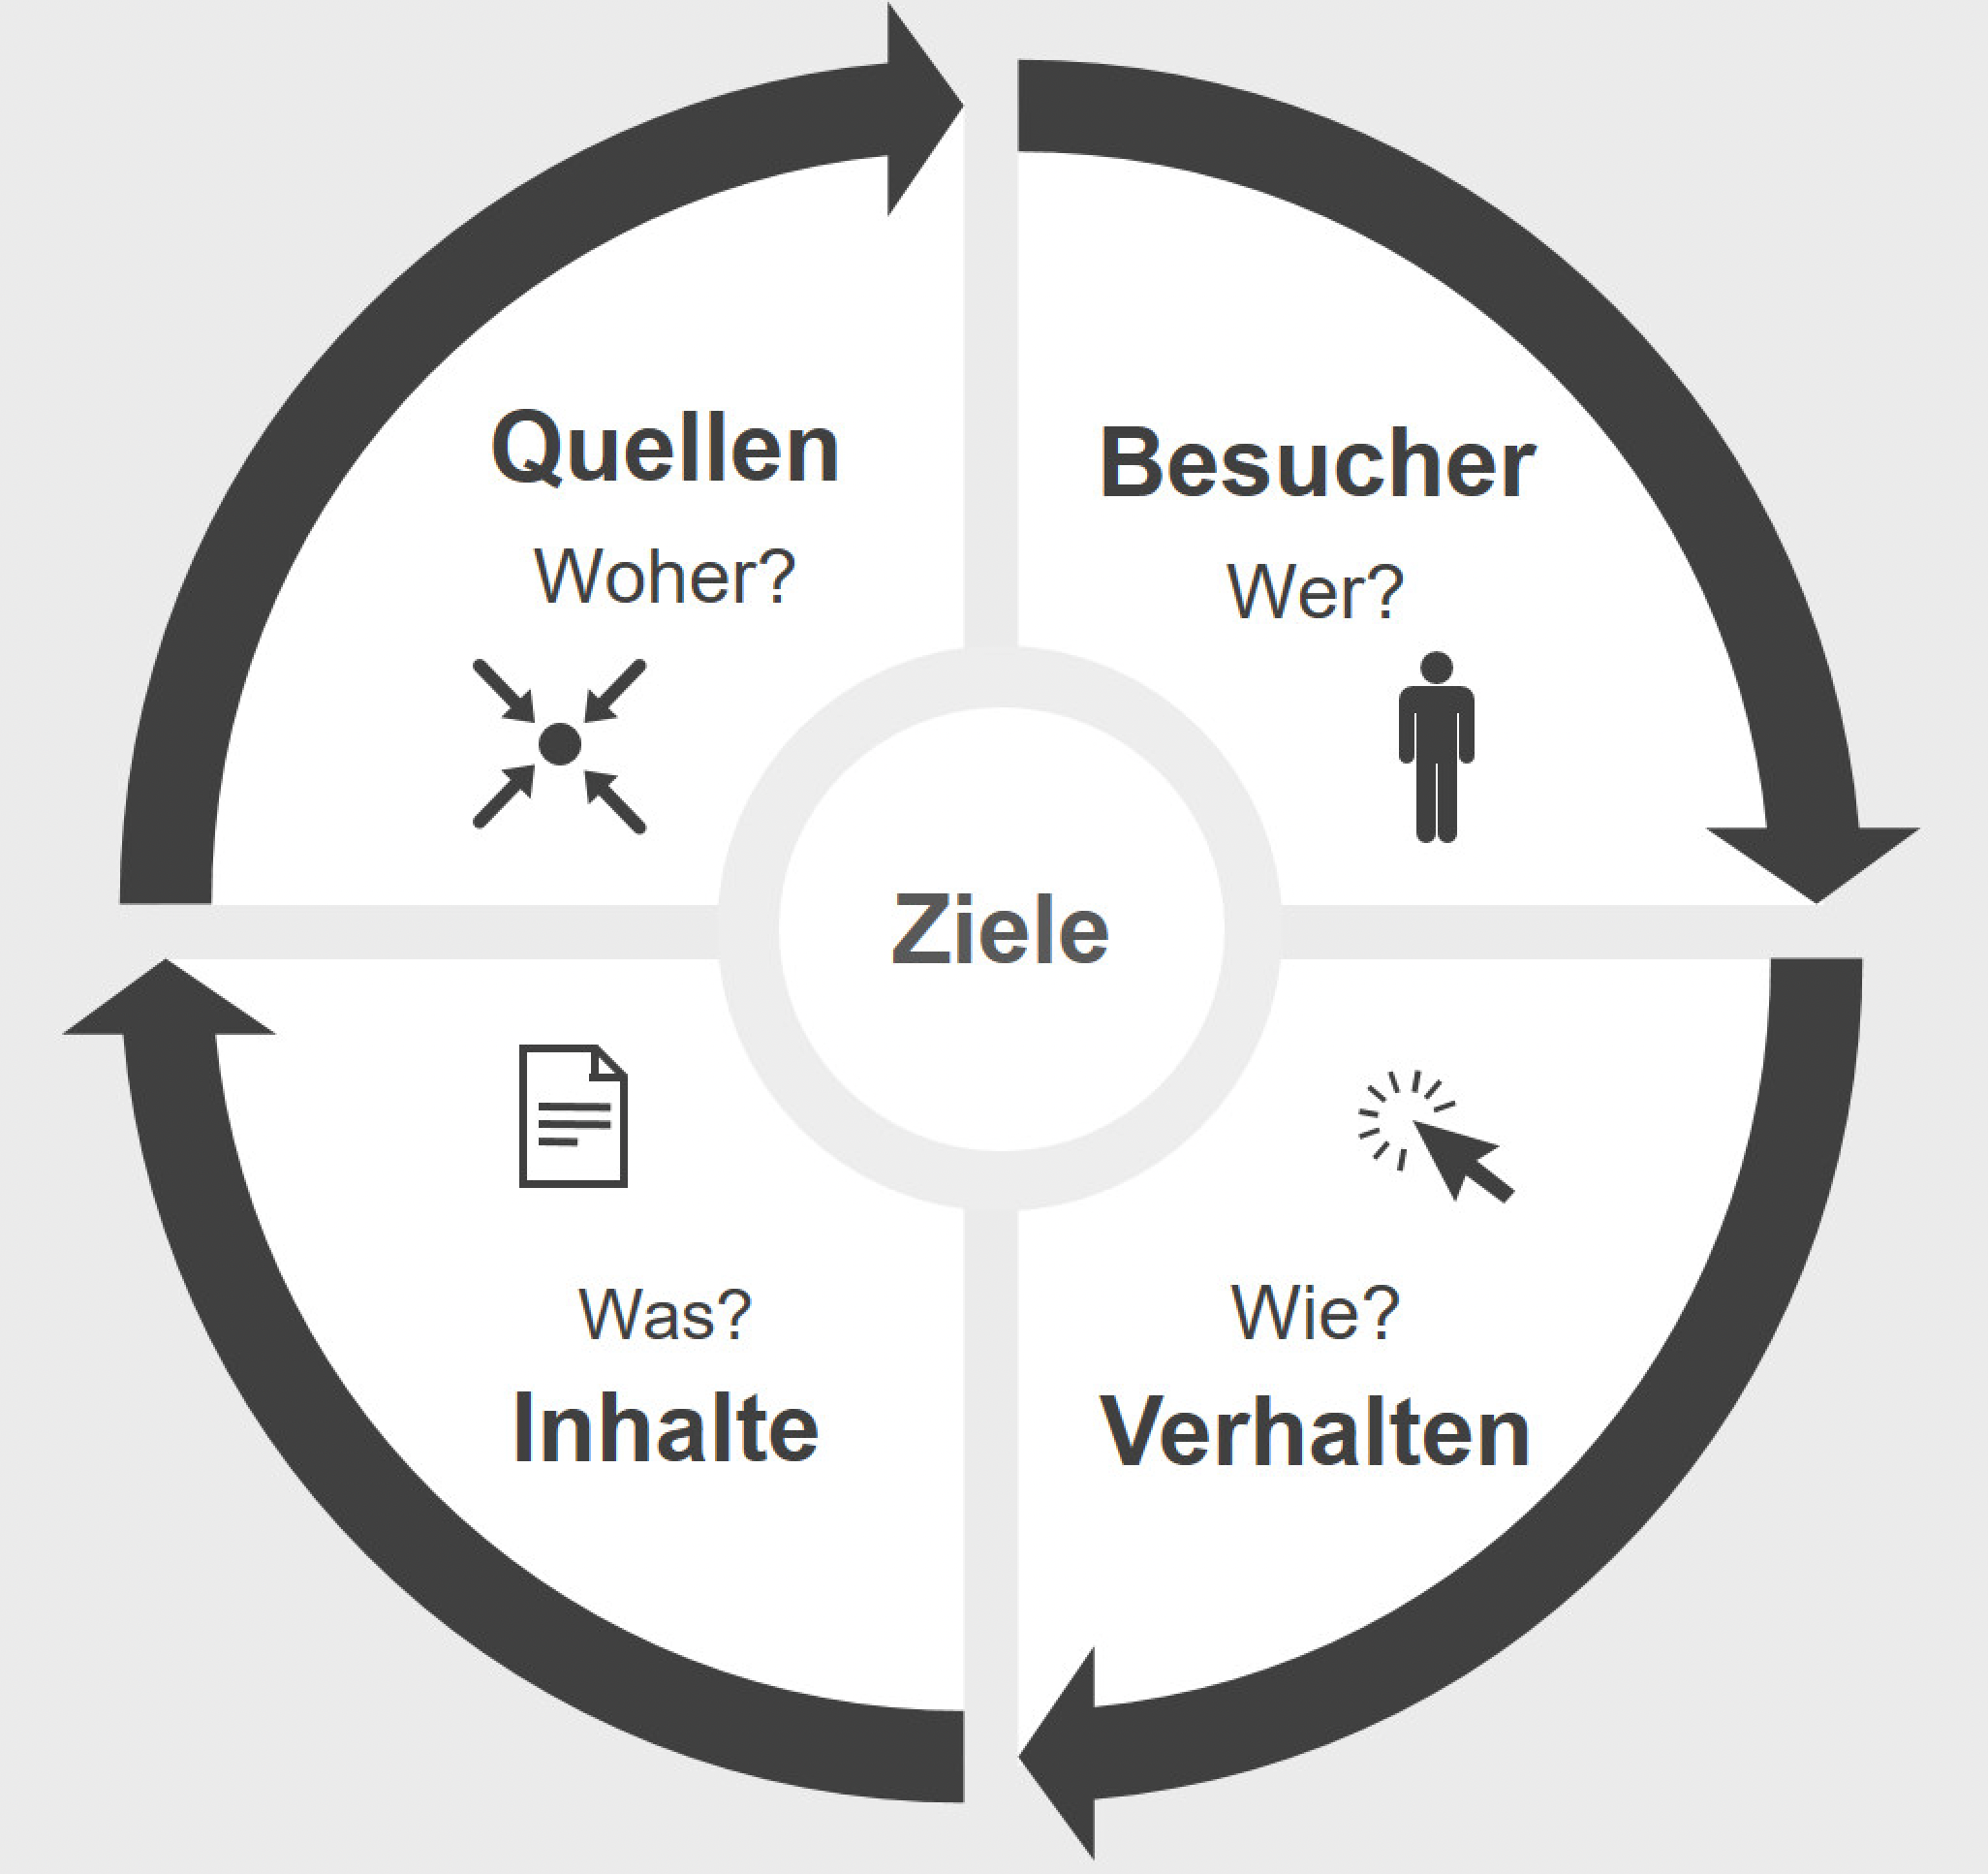
\includegraphics[width=0.6\textwidth, keepaspectratio]{images/dimensionen.png}
    \caption{Metriken beleuchten hauptsächlich vier Dimensionen einer Website \parencite[Kap.5.7]{Hassler2019}}
    \label{fig:dimensionen}
\end{figure}


Zusätzlich zu diesen Dimensionen beschreibt Hassler in seinem Buch \glqq Digital und Web Analytics\grqq{} die Wichtigkeit von Zielen bei der Webanalyse. Ziele sind essenziell, um den Erfolg der Website zu bewerten und sollten so gewählt werden, dass sie konkrete, messbare Nutzerinteraktionen widerspiegeln. Somit bieten Ziele einen Orientierungspunkt, um das Verhalten der Besucher besser einschätzen zu können. Um die Zielerreichung messbar zu machen, kommen in der Webanalyse oftmals sogenannte Konvertierungen (engl. Conversions) zum Einsatz. Bei einer Conversion handelt es sich um eine Nutzerinteraktion, welche aus Sicht des Betreibers der Website als erwünschtes Verhalten gilt. \parencite[Kap.13]{Hassler2019}

Die Conversion-Rate setzt die Anzahl der Besucher einer Website ins Verhältnis zu den tatsächlich erzielten Conversions und wird in Prozent angegeben. Da bei einer Conversion-Rate Messgrößen mit einem konkreten Ziel verknüpft werden, spricht man hierbei von einem KPI. \parencite{RyteConversion}

Da es sich bei der Website \textit{evaschiffmann.de} nicht um eine E-Commerce Website handelt, sind die Ziele keine kommerziellen. Trotzdem lassen sich Ziele definieren, welche einen Aufschluss darüber liefern, wie oft Besucher mit den Kernelementen der Website interagieren.

Die Tabelle~\ref{tab:analysewerte} gibt einen Überblick über alle zu erfassenden Analysewerte und ordnet diese den jeweiligen Dimensionen zu. In der letzten Spalte wird zudem angegeben, ob es sich bei dem Analysewert um eine Metrik oder einen KPI handelt. Wie diese Metriken und KPIs im Detail funktionieren, wird in Kapitel~\ref{ch:implementierung} beschrieben.

\begin{table}[H]
    \centering
    \begin{tabularx}{\textwidth}{l l l}
        \hline
        \textbf{Analysewert} & \textbf{Dimension} & \textbf{Art der Daten} \\
        \hline
        Ranking der Referer Seiten & Quellen & Metrik \\
        Verteilung der Traffic Quellen & Quellen & Metrik \\
        Verteilung der Gerätetypen & Besucher & Metrik \\
        Anzahl der Besuche & Besucher & Metrik \\
        Anzahl der wiederkehrenden Besucher & Besucher & Metrik \\
        Anteil der wiederkehrenden Besucher & Besucher & Metrik \\
        Anzahl der einmaligen Besucher & Besucher & Metrik \\
        Seitenaufrufe nach Häufigkeit & Inhalte & Metrik \\
        Ranking der am häufigsten aufgeklappten Überschriften & Inhalte & Metrik \\
        Verweildauer & Verhalten & Metrik \\
        Bounce-Rate & Verhalten & Metrik \\
        Conversion: min. eine Tagebuchseite geöffnet & Ziel & KPI \\
        Conversion: min. drei Tagebuchseiten geöffnet & Ziel & KPI \\
        Conversion: min. eine Überschrift aufgeklappt & Ziel & KPI \\
        Conversion: min. drei Überschriften aufgeklappt & Ziel & KPI \\
        \hline
    \end{tabularx}
    \caption{Analysewerte und ihre Klassifizierung nach Dimension und Art}
    \label{tab:analysewerte}
\end{table}

Zusätzlich zu diesen Analysewerten soll auch die Möglichkeit bestehen, eine individuelle Nutzersitzung nachzuvollziehen. Dieser Analyseaspekt gehört sowohl zur Dimension Inhalte, da nachvollzogen werden kann, welche Seiteninhalte aufgerufen wurden, als auch zur Dimension Verhalten, da die Interaktionen wie Klickverläufe und Seitenaufrufe erfasst werden.

\section{Datenerfassung}
\label{sec:Datenerfassung}
\subsection{Logfile-Analyse}
\label{sec:logfiles}
Die ersten Webanalyse-Tools basierten auf der Analyse von Logdateien (engl. Logfiles). Jedes Mal, wenn ein Nutzer eine Webseite aufruft, sendet der Browser eine Anfrage an den Webserver, um die Inhalte der Seite zu laden. Der Webserver zeichnet jede dieser Anfragen, auch \glqq Hit\grqq{} genannt, in einer Logdatei auf. \parencite[S.8]{Dykes2014}

Diese Logfiles werden in Form von Textdateien gespeichert und bieten eine strukturierte Übersicht über alle Interaktionen auf dem Server. Die Erstellung von Logfiles erfolgt automatisch, indem der Webserver Interaktionen zwischen Nutzer und Webseite aufzeichnet. Sobald ein Nutzer eine Webseite aufruft, sendet der Browser mehrere Anforderungen (engl. Requests) an den Server, um die verschiedenen Elemente der Seite wie Texte, Bilder oder Skripte zu laden. Der Server liefert daraufhin die angeforderten Inhalte zurück (engl. Responses) und speichert diese Vorgänge zeitgleich in einer Logdatei. Diese Dateien, die in der Regel täglich neu generiert werden, dienen als Quelle für die Analyse von Zugriffen auf die Website. \parencite[Kap.2.2]{Hassler2019}

Im Listing~\ref{lst:logfile} ist ein Beispiel eines Logfile-Eintrags im Common Logfile Format (CLF) zu sehen:

\lstinputlisting[caption=Logfile-Eintrag im CLF \parencite{ApacheLogFiles}, label={lst:logfile}, language=Apache]{listings/logfile_entry.txt}

Aus diesem Beispiel eines Eintrags lassen sich folgende Informationen in entsprechender Reihenfolge entnehmen \parencite{ApacheLogFiles}:

\begin{itemize}
    \item IP-Adresse des Aufrufenden
    \item Identitätskennzeichen
    \item Authentifizierter Benutzername
    \item Aufrufdatum und Zeit
    \item URL der aufgerufenen Datei
    \item HTTP-Anfrage
    \item Ergebnis des Aufrufs (Status)
    \item Größe der zurückgegebenen Datei
\end{itemize}

Zusätzlich wird in der Logfile auch die Aufrufmethode (z. B. \texttt{GET} oder \texttt{POST}) gespeichert. Diese Angabe ist jedoch für eine spätere Analyse oft weniger relevant \parencite[Kap.2.2]{Hassler2019}. Der Vorteil dieser Methode ist, dass die Datenerfassung unabhängig von Client-Technologien abläuft, da diese serverseitig erfolgt und keine zusätzlichen Technologien wie JavaScript notwendig sind \parencite{RyteLogFiles}. Ein Nachteil bei der serverseitigen Erfassung von Nutzerdaten ist, dass clientseitige Informationen, welche nicht an den Webserver übertragen werden, nicht erfasst werden können. Somit werden Interaktionen mit der Website, welche keine Request auslösen nicht protokolliert und können nicht ausgewertet werden. Zudem können Seitenaufrufe, welche aus dem Browser-Cache geladen werden, nicht in den Logfiles erfasst werden. Ein Verfahren, welches für dieses Problem Abhilfe schafft und Nutzer einer Website nicht aus der Sicht des Servers, sondern aus Sicht des Clients betrachtet, ist das sogenannte Page-Tagging. \parencite{CounterCodePageTagging}, \parencite{CounterCodeLogFiles}

\subsection{Page Tagging}
\label{sec:pagetagging}
Unter Page-Tagging versteht man die Einbindung eines kurzen Codeausschnittes (engl. Snippet) in den HTML-Code einer Webseite, um Nutzerdaten zu erfassen. Dieses Snippet ist meistens in der Programmiersprache Javascript geschrieben. Das Snippet ermöglicht die Datenerfassung, indem es eine Javascript-Bibliothek herunterlädt, die im Cache-Speicher des Webbrowsers hinterlegt wird, um bei zukünftigen Seitenaufrufen schneller geladen zu werden. Nachdem das Page-Tag die Bibliothek geladen hat, wird der enthaltene Programmcode ausgeführt, um verschiedene Daten aus dem Browser zu sammeln. \parencite[S.70-71]{Dykes2014}

Es können zum einen Daten abegerufen werden, welche per Browser Object Model (BOM) bezüglich der Einstellungen für den Webbrowser zu Verfügung stehen und zum anderen auch Informationen, welche das Document Object Model (DOM) enthält. Hierbei lassen sich unter anderem folgende Informationen per Page-Tag sammeln \parencite[Kap.2.3]{Hassler2019}:

\begin{itemize}
    \item Interaktionen mit Multimedia-Dateien
    \item Verweise in Form von Links
    \item Titel der Seite
    \item Tastatureingaben
    \item Bildschirmauflösung
    \item Cookies
    \item Alle Informationen, welche auch Logfiles liefern
\end{itemize}

Um die gesammelten Daten an den Webserver zu übertragen, wird ein Bild in der Größe eines Pixels erzeugt, weshalb dieses Verfahren ebenfalls als Pixel-Tracking bezeichnet wird \parencite[Kap.2.3]{Hassler2019}. Der Webbrowser erkennt dieses Bild als fehlenden Inhalt an, der geladen werden muss und sendet eine HTTP-Anfrage um es abzurufen. Diese Anfrage wird auch als Image-Request bezeichnet und enthält alle zuvor gesammelten Daten als Parameter in der URL. Die Image-Request wird allerdings nicht an den Webserver gesendet, auf welchem die Website hinterlegt ist, sondern an einen dedizierten Datensammlungsserver. Wurden die Daten vom Datensammlungsserver empfangen, werden die Parameter aus der URL extrahiert und in einer Datenbank gespeichert. Anschließend können die Daten von einer Analyse-Engine verarbeitet werden, um zusätzliche Einsichten in das Nutzerverhalten zu gewinnen. Neben der Verarbeitung der Daten kann der Datensammlungsserver in der HTTP-Antwort auch einen Cookie setzen. Dieser Cookie enthält eine eindeutige Kennung (Visitor-ID), die es ermöglicht, dass Gerät des Nutzers bei zukünftigen Besuchen wiederzuerkennen und gesammelte Daten mit diesem zu verknüpfen. \parencite[S.70-72]{Dykes2014}

\subsection{Events}
\label{sec:events}
Ein Event beschreibt eine gezielte Aktion, die auf einer Webseite durch einen Nutzer ausgelöst wird. Diese Aktionen werden entweder vom Browser oder vom Server protokolliert und mit einem Zeitstempel versehen. Events können unter anderem das Einblenden von Werbeanzeigen, Änderungen in Formularfeldern oder das Abspielen von Videos sein. \parencite[S.13]{WAA2008}

Für das Bildungsportal \textit{evaschiffmann.de} werden Events somit verwendet, um Interaktionen mit Video- und Audioelementen zu erkennen. Ebenso werden Events genutzt, um das Auf- und Zuklappen von Überschriften zu erfassen, da Events ohne ein Neuladen der Seite ausgelöst werden können \parencite{ATInternet}.

\subsection{Datenschutz und rechtliche Anforderungen}
\label{sec:datenschutz}
Logfiles und das Page-Tagging sorgen dafür das die Daten erfasst werden können. Im Umgang mit diesen Daten muss allerdings einiges beachtet werden, um den gesetzlichen Datenschutzanforderungen gerecht zu werden. Im Folgenden werden die rechtlichen Aspekte und deren Auswirkungen auf die Webanalyse näher beleuchtet.

Art. 6 Abs. 1 der DSGVO gibt vor, dass die Verarbeitung personenbezogener Daten nur rechtmäßig ist, wenn sie auf einer rechtlichen Grundlage beruht. Im Kontext der Webanalyse ist die Einwilligung (Art. 6 Abs. 1 lit. a) relevant, welche vor der Datenerhebung eingeholt werden muss. Alternativ kann ein berechtigtes Interesse des Verantwortlichen (Art. 6 Abs. 1 lit. f) geltend gemacht werden, sofern die Interessen der Nutzer gewahrt bleiben. \parencite{DSGVO}

Die rechtlichen Anforderungen der DSGVO haben direkte Auswirkungen auf die Gestaltung und den Betrieb der Webanalyse. Als wichtige Aspekte gelten \parencite[Kap.2.4]{Hanschke2020}:

\begin{itemize}
    \item \textbf{Transparenz:} Nutzer müssen darüber informiert werden, welche Daten erfasst werden und zu welchem Zweck.
    \item \textbf{Datenminimierung:} Analysesysteme sollten nur die für den jeweiligen Zweck erforderlichen Daten sammeln.
    \item \textbf{Einwilligung:} Die Verarbeitung personenbezogener Daten geschieht oft durch den Einsatz von Cookies. Hierzu muss die Einwilligung der Nutzer eingeholt werden. 
\end{itemize}

Die IP-Adresse wird von der DSGVO als personenbezogenes Datum eingestuft, da sie in Kombination mit weiteren Informationen eine Identifizierung der Person ermöglichen kann. Analytics-Systeme müssen daher Maßnahmen ergreifen, um die Verarbeitung der IP-Adressen DSGVO-konform zu gestalten. Häufig wird die IP-Adresse anonymisiert, bevor sie gespeichert oder weiterverarbeitet wird. Tools wie Google Analytics und Matomo bieten eine Funktion zur IP-Anonymisierung, bei der die letzten Stellen der IP-Adresse entfernt werden. \parencite{eRecht23} \parencite{MatomoGDPR} 

Cookies werden in der Webanalyse dazu verwendet, Nutzer über verschiedene Sitzungen hinweg zu identifizieren \parencite[Kap.2.2]{Hassler2019}. Damit dies DSGVO-konform geschehen kann, muss ein explizites Opt-In, also eine Einverständniserklärung durch den Nutzer erfolgen \parencite[Kap.2.4]{Hanschke2020}. Laut Art. 7 Abs. 3 der DSGVO müssen Nutzer die Möglichkeit haben, ihre Einwilligung jederzeit zu widerrufen \parencite{DSGVO}. 

\section{Anforderungen an das Webanalyse-Tool}
\label{sec:anforderungenWebanalyseTool}
Es gibt eine große Anzahl von Webanalyse-Tools, welche sich in ihren Funktionen, Kosten und technischen Ansätzen erheblich unterscheiden \parencite[S.244]{Rittgerberger2016}. Grundsätzlich ist das Page-Tagging besser geeignet, um detaillierte Informationen über das Nutzerverhalten auf Webseiten zu erfassen \parencite[Kap.2.5.3]{Hassler2019}. Logfiles hingegen wurden ursprünglich zur technischen Überwachung entwickelt und enthalten nicht die hierfür erforderlichen Daten \parencite[Kap.2.5.3]{Hassler2019}. Somit und mit den Erkenntnissen aus Kapitel~\ref{sec:pagetagging} wird deutlich, dass das Page-Tagging nicht nur umfangreiche Nutzerdaten liefert, sondern auch alle Informationen abdeckt, die durch die Analyse von Logfiles erfasst werden können. Weshalb bei der Auswahl einer Tool-Lösung ebenfalls darauf geachtet wird, dass die Daten per Page-Tagging beziehungsweise per Events erhoben werden.

Neben der Methode der Datenerhebung wurden noch weitere Anforderungen an das Webanalyse Tool definiert:

\begin{itemize}
    \item \textbf{Datenschutz und DSGVO-Konformität:} Wie im vorherigen Kapitel erläutert, sind Datenschutz und die Einhaltung der DSGVO grundlegende Anforderungen an ein Webanalyse-Tool. Somit muss dieses in der Lage sein, die geltenden Datenschutzgesätze einzuhalten.
    \item \textbf{Sicherheit und Zugriffskontrolle:} Es muss sichergestellt werden, dass nur authentifizierte Benutzer Zugriff auf die Anwendung haben. Somit soll die Weboberfläche ausschließlich über HTTPS erreichbar gemacht werden. Für die Authentifizierung wird eine Rollenbasierte Zugriffskontrolle (engl. Roll based Access Controll (RBAC)) benötigt.
\end{itemize}

\section{Matomo als Webanalyse-Tool}
Google Analytics (GA) ist mit einem Marktanteil von 82,0 \% unter den Websites, welche Webanalyse-Tools verwenden, dass mit Abstand am weitesten verbreitete Tool \parencite{W3Techs2025}. GA hat allerdings insbesondere in Europa stark an Akzeptanz verloren, da es wiederholt in Konflikt mit den Vorgaben der DSGVO geraten ist \parencite{Förster2024}. Seit dem Ende des EU-US Privacy Shield ist die rechtliche Grundlage für die Übertragung von Nutzerdaten in die USA weggefallen, weshalb Google Analytics mehrfach als nicht datenschutzkonform eingestuft wurde \parencite{Förster2024}.

Auf Grundlage dessen ist es keine Option, GA für das Sammeln von Nutzerdaten auf dem Bildungsportal zu verwenden. Ein Tool, welches eine datenschutzkonforme Erhebung der Nutzerdaten ermöglicht und ebenfalls kostenlos auf einem eigenen Server gehostet werden kann, (engl. On-Premise) ist Matomo. \parencite{Förster2024}, \parencite{MatomoFree}

Matomo wurde bereits 2007 gegründet und war zunächst unter dem Namen Piwik bekannt. Durch die langjährige Marktpräsenz hat sich eine umfassende Wissensbasis entwickelt, welche sowohl die Matomo Knowledge Base als auch eine Developer-Dokumentation umfasst. Ergänzt wird diese durch eine Vielzahl an praxisnahen Guides, Tutorials und Best-Practice-Beispielen. Somit bietet Matomo im Vergleich zu dem Tool PostHog, welches erst 2024 eine Webanalyse-Funktion eingeführt hat, eine größere Wissensbasis, was die Einarbeitung in das Tool erheblich erleichtert. Daher wird das Webanalyse-Tool Matomo anstelle von PostHog gewählt. \parencite{MatomoKnowledgeBase}, \parencite{Förster2024}, \parencite{MatomoDevelop}

Matomo sorgt dafür, dass Analysedaten auf einer Website gesammelt, gespeichert und in Form von Bereichten (engl. Reports) oder direkt über Anfragen an die Matomo Datenbank ausgeliefert werden können \parencite{MatomoHowItWorks}. Das Tool ist Open-Source und kann auf verschiedenen Betriebsystemen wie Linux, Windows und macOS installiert werden \parencite{MatomoRequirements}. Alternativ dazu steht ein offizielles Docker-Image für die Bereitstellung in Container-Umgebungen zur Verfügung \parencite{MatomoDocker}. Matomo benötigt eine MySQL oder MariaDB Datenbank, um die Analysedaten zu speichern \parencite{MatomoRequirements}. 

Um die Datengenauigkeit zu gewährleisten, verzichtet Matomo vollständig auf Begrenzungen bei der Anzahl getrackter Seitenaufrufe, Besuche oder Events. Die Auswertungen basieren auf vollständigen Rohdaten, ohne den Einsatz von Data Sampling, also einem Verfahren, bei dem aus Effizienzgründen lediglich ein Teil der gesammelten Daten analysiert wird, was zu einer verminderten Genauigkeit führen kann. \parencite{PiwikProDataSampling}, \parencite{MatomoDataLimits}

Nachdem Matomo installiert und konfiguriert wurde, kann das Page-Tag in den Quellcode der Website eingebunden werden, um die Erfassung und Übertragung von Nutzerdaten an den Matomo-Server (\texttt{matomo.php}) zu ermöglichen. Dabei wird der enthaltene Code bei jedem Seitenaufruf ausgeführt und sendet die gesammelten Daten an den Server. Das Page-Tag verweist auf die Datei \texttt{matomo.js}, welche die Tracking-Logik enthält. Nach der Datenerfassung sendet \texttt{matomo.js} die gesammelten Informationen in Form einer HTTP-Request an die Tracking-API \texttt{matomo.php} der Matomo-Instanz. Diese Instanz nimmt die Anfragen entgegen, verarbeitet diese und speichert die Rohdaten anschließend in der zugrunde liegenden Datenbank. Damit die Daten effizient abgerufen werden können, durchläuft Matomo einen Archivierungsprozess, bei dem die Rohdaten aggregiert und für die Erstellung von Reports optimiert werden. Diese Reports können über die Matomo Reporting API abgerufen werden. \parencite{MatomoHowItWorks}, \parencite{MatomoTrackingClient}

Matomo ermöglicht es außerdem eigenen Events zu definieren. Jedes Event besteht aus einer Kategorie und einer Aktion. Optional können Events ebenfalls noch einen Namen und einen Wert enthalten \parencite{MatomoEvent}. Ein Beispiel für eine Funktion, welche ein solches Event auslöst ist in Listing~\ref{lst:exampleEvent} zu sehen: 

\begin{figure}[H]
    \centering
    \begin{minipage}{\textwidth}
        \lstinputlisting[
            caption=Funktion zur Erfassung eines Matomo-Events beim Aufruf eines Tagebucheintrags,
            label={lst:exampleEvent},
        ]{listings/exampleEvent.js}
    \end{minipage}
\end{figure}

In dem Beispiel aus Listing~\ref{lst:exampleEvent} wird exemplarisch gezeigt, wie ein Event aufgebaut ist, welches erfasst, wenn ein Nutzer einen Tagebucheintrag öffnet. Die Methode \texttt{\detokenize{_paq.push([])}} weist Matomo an, Daten in die Plattform zu übertragen, während \glqq trackEvent\grqq{} den Typ der gesendeten Daten definiert. Matomo erkennt die folgenden Parameter als Event-Attribute \parencite{MatomoEvent}:

\begin{itemize}
    \item  \glqq DiaryEntry\grqq{} ist die Kategorie, über welche alle Events im Zusammenhang mit Tagebucheinträgen gruppiert werden können.
    \item \glqq DiaryEntryOpened\grqq{} ist die Aktion, die angibt, dass der Eintrag geöffnet wurde.
    \item \glqq DiaryEntryName\grqq{} ist der Name, der den spezifischen Titel oder die ID des geöffneten Tagebucheintrags enthält.
\end{itemize}

Um nun das Event an der entsprechenden Stelle auszulösen, kann die Funktion innerhalb des entsprechenden HTML-Elementes eingebunden werden. Siehe Listing~\ref{lst:exampleEventCall}: 

\begin{figure}[H]
    \centering
    \begin{minipage}{\textwidth}
        \lstinputlisting[
            caption=Auslösen eines Matomo-Events beim Anklicken eines Tagebucheintrags,
            label={lst:exampleEventCall},
        ]{listings/exampleEventCall.html}
    \end{minipage}
\end{figure}

Hierbei wird das in Listing~\ref{lst:exampleEvent} definierte Event innerhalb des HTML-Elementes \texttt{<a>} ausgelöst und über das \texttt{onclick}-Attribut wird die Javascript-Funktion aufgerufen.

Um sicherzustellen, dass nur authentifizierte Benutzer Zugriff auf das Tool haben, sind eine Benutzerauthentifizierung und eine verschlüsselte Verbindung zur Benutzeroberfläche notwendig. In Matomo gibt es verschiedene Benutzerrollen mit jeweils unterschiedlichen Berechtigungen, vom einfachen Lesezugriff bis hin zur vollständigen Verwaltung von Websites und Konfigurationen \parencite{MatomoRBAC}. Für das Anlegen eines neuen Benutzerkontos wird eine gültige E-Mail-Adresse benötigt, die im Anmeldeprozess bestätigt werden muss. Wie Matomo ausschließlich über HTTPS erreichbar gemacht wird, wird in Kapitel~\ref{ch:implementierung} beschrieben.  
    \chapter{Dashboard Visualisierung} % 5-6 Seiten? 
\label{ch:auswahl}
Im vorherigen Kapitel wurde beleuchtet, wie Nutzerdaten erfasst werden können. Hierfür wurden die relevanten Analysewerte für das Bildungsportal definiert und verschiedene Methoden der Datenerhebung sowie deren DSGVO-konforme Umsetzung erläutert. Um die gesammelten Daten strukturiert und übersichtlich darzustellen und der Professur für Geschichtsdidaktik eine fundierte Grundlage für datenbasierte Erkenntnisse zu bieten, sollen die Analysewerte visuell auf einem Dashboard aufbereitet werden. Dazu werden zunächst technische-funktionale Anforderungen sowie Usability- und Design Anforderungen an das Dashboard definiert. Im Laufe des Kapitels wird zunächst darauf eingegangen, wie die Usability- und Design Anforderungen umgesetzt werden können. Ebenso wird die Struktur sowie der Aufbau des Dashboards bestimmt. Es werden geeignete Visualisierungsmethoden für die Analysewerte definiert und schlussendlich wird Grafana als Visualisierungslösung vorgestellt. Hierbei wird auf das Unterkapitel~\ref{sssec:technfunk} Bezug genommen und beschrieben wie die technisch-funktionalen Anforderungen in Grafana realisiert werden können.

\section{Anforderungen an das Dashboard}
\label{sec:anforderungen}
\subsection{Technisch-funktionale Anforderungen das Dashboard}
\label{sssec:technfunk}
Die technisch-funktionalen Anforderungen sollen bei der Auswahl einer Dashboard Lösung Orientierung geben, welche Funktionen das Tool bereitstellen muss und welche technologischen Rahmenbedingungen erfüllt sein müssen, um eine effiziente Nutzung zusammen mit Matomo zu gewährleisten. Diese Anforderungen sind: 
\begin{itemize}
    \item \textbf{Datenintegration und Aggregation:} Das Dashboard-Tool soll in der Lage sein, die gesammelten Daten von Matomo zu beziehen und zu aggregieren. Außerdem sollen die per Webanalyse-Tool erfassten Daten automatisch aktualisiert werden, entweder in definierten Intervallen oder in Echtzeit.
    \item \textbf{Filtermöglichkeiten:} Es soll die Möglichkeit geboten werden, die erhaltenen Daten zu filtern. Hierbei soll eine Filterung nach Zeitraum und auch eine Filterung nach Unterseite möglich sein, sodass relevante Daten für einzelne Unterseiten analysiert werden könnnen. 
    \item \textbf{Sicherheit und Zugriffskontrolle:} Ebenfalls wie für Matomo, muss auch für Grafana sichergestellt werden, dass nur authentifizierte Benutzer Zugriff auf das Dashboard haben. Somit soll das Dashboard ebenfalls wie Matomo über HTTPS erreichbar gemacht werden. Für die Authentifizierung wird eine ebenfalls eine RBAC benötigt.
\end{itemize}

\subsection{Usability- und Design Anforderungen das Dashboard}
\label{sssec:usability}
Neben technischen Aspekten soll die Benutzerfreundlichkeit gewährleistet sein. Ebenfalls wird auf eine sinnvolle Anordnung und eine geeignete Darstellung für die Analysewerte geachtet. Wichtige Anforderungen sind hierbei:
\begin{itemize}
    \item \textbf{Anordnung der Inhalte:} Die Analysewerte sollen so dargestellt werden, dass verwandte Analysewerte auch im Dashboard nebeneinander zu finden sind.
    \item \textbf{Visualisierung der Inhalte:} Ein einheitliches Farbschema soll die Orientierung erleichtern. Ebenfalls sollen positive und negative Trends einer KPI auf dem ersten Blick zu erkennen sein. Außerdem soll für gleiche Arten von Analysewerten eine konsistente Visualisierungsform genutzt werden, um eine einheitliche Darstellung im Dashboard zu gewährleisten und Verwirrungen zu vermeiden.
    \item \textbf{Responsives Design:} Das Dashboard soll auf verschiedenen Geräten und Bildschirmgrößen benutzerfreundlich dargestellt werden. Die Darstellung soll sich automatisch an unterschiedliche Bildschirmbreiten anpassen, sodass eine Nutzung auf verschiedenen Endgeräten möglich ist.
\end{itemize}

\section{Struktur und Aufbau des Dashboards}
Bei der Gestaltung eines Dashboards ist es sinnvoll, verwandte Daten zu gruppieren, um eine klare Struktur und eine bessere Übersichtlichkeit zu gewährleisten. Besonders bei einer großen Anzahl an Kennzahlen hilft diese Form der Gruppierung dabei, die relevanten Informationen gezielt darzustellen, ohne den Gesamtüberblick zu verlieren. \parencite[Kap.14.3]{Hassler2019}

Ebenso kann, laut Stephen Few, die Möglichkeit zur Navigation zwischen unterschiedlichen Dashboardseiten (engl. Screens) eine sinnvolle Funktion sein. Die Aufteilung der Analysewerte in solche Screens ist allerdings nur dann sinnvoll, wenn dadurch keine Daten fragmentiert werden, welche eigentlich zusammenhängend betrachtet werden sollten. Andernfalls kann eine solche Aufteilung die Effizienz eines Dashboards erheblich einschränken, da zusammengehörige Informationen schwerer in einem sinnvollen Kontext betrachtet werden können. \parencite[Kap.3.1.1]{Few2006}

Auch die Notwendigkeit, innerhalb eines Dashboards vertikal oder horizontal zu scrollen, kann die Übersichtlichkeit und Effizienz beeinträchtigen. Laut Few führt dies dazu, dass Nutzer nicht auf einen Blick alle wichtigen Daten erfassen können und häufig nicht bemerken, dass sich weitere relevante Informationen außerhalb des sichtbaren Bereichs befinden. Elemente, die nicht sofort sichtbar sind, werden oft als weniger wichtig wahrgenommen oder gar übersehen, was die Effektivität eines Dashboards erheblich einschränken kann. \parencite[Kap.3.1.1]{Few2006}

Für das Bildungsportal \textit{evaschiffmann.de} bietet es sich an, die Analysewerte auf einer Haupt-Dashboardseite zusammenzuführen, da diese alle der Analyse des Bildungsportals dienen. Die detaillierte Auswertung einzelner Nutzersitzungen erfordert hingegen deutlich mehr Platz, da je nach Sitzungsdauer und Anzahl der Aktionen eine große Menge an Daten erfasst werden. Um unnötiges Scrollen zu vermeiden und die Übersichtlichkeit zu wahren, wird diese Darstellung daher auf eine separate Dashboard-Seite ausgelagert.

\subsection{Anordnung der Inhalte}
Um nun die Analysewerte auf der Haupt-Dashboardseite so anzuordnen, dass Analysewerte, welche dem selben Kontext dienen nah bei einander angezeigt werden, empfiehlt sich eine Gruppierung nach Untersuchungsthema \parencite[Kap.14.3.1]{Hassler2019}. Diese Untersuchungsthemen sind die in Kapitel~\ref{sec:kpis} erläuterten Dimensionen. Somit werden die Analysewerte auf dem Dashboard so angeordnet wie in Abbildung~\ref{fig:dimensionen} zu erkennen. Metriken zu den Quellen sollen oben links dargestellt werden, Metriken zu den Besuchern oben rechts. Die Inhalte sind unten links zu finden und der Bereich unten rechts soll Aufschluss über das Verhalten der Nutzer geben.

\section{Visualisierung der Inhalte}
\label{sec:Visualisierungsmethoden}
Nachdem die Dashboardstruktur sowie die Anordnung der Inhalte festgelegt wurden, sollen nun geeignete Visualisierungsformen für die Analysewerte bestimmt werden. 
Ein wesentlicher Bestandteil einer effektiven Datenvisualisierung ist eine eindeutige und aussagekräftige Beschriftung. Titel dienen dazu, den Inhalt einer Abbildung prägnant zusammenzufassen und die beabsichtigte Botschaft klar zu vermitteln. Laut Wilke sollte eine Abbildung genau einen Titel besitzen, dieser kann entweder direkt in die Visualisierung integriert werden oder als erstes Element in einer Bildunterschrift angegeben werden. Außerdem sollten die Achsen von Diagrammen immer mit einer entsprechenden Beschriftung versehen sein, welche bei der Zuordnung der Analysewerte hilft. \parencite[Kap.22]{Wilke}

Um Zahlenwerte, welche für bestimmte Kategorien erfasst werden aussagekräftig darzustellen, ist ein Balkendiagramm gut geeignet \parencite[Kap.5]{Wilke}. Hierzu zählt die Metrik \glqq Seitenaufrufe nach Häufigkeit\grqq{}. Dabei stellen die Namen der einzelnen Unterseiten die Kategorien dar, während die zugehörigen Zahlenwerte die Anzahl der Seitenaufrufe repräsentieren.

Die Metriken \glqq Verteilung der Traffic Quellen\grqq{} und \glqq Verteilung der Gerätetypen\grqq{} fallen ebenfalls in diese Kategorie. Da es sich hierbei allerdings um Proportionen handelt und aufgezeigt werden soll, wie die Verteilung über die gesamte Menge ist, ist hierfür ein Kreisdiagramm die bessere Wahl \parencite[Kap.5]{Wilke}.

Da für die Metriken \glqq Ranking der Referer Seiten\grqq{} und dem \glqq Ranking der am häufigsten aufgeklappten Überschriften\grqq{} jeweils Kategorien mit mehreren Zahlenwerten erfasst werden, ist eine tabellarische Darstellung aufgrund der besseren Übersichtlichkeit sinnvoller \parencite{Auditrium}. Für das \glqq Ranking der Referer Seiten\grqq{} soll neben der Anzahl der Besuche über einen bestimmten Referer auch die Anzahl der Beusche erfasst werden, in denen Nutzer nur eine einzige Aktion auf der Website durchgeführt haben. Für das \glqq Ranking der am häufigsten aufgeklappten Überschriften\grqq{} sollen neben dem Titel und der Häufigkeit des Aufklappens auch die Gesamtanzahl aller aufgeklappten Überschriften angezeigt werden.

Einfachen numerischen Metriken, die lediglich aus einem einzelnen quantitativen Wert bestehen, wird keine explizite Visualisierungsform zugewiesen, da sie keine vergleichenden oder relationalen Darstellungen erfordern. Für die Metriken \glqq Anzahl der Besuche\grqq{}, \glqq Anzahl der wiederkehrenden Besucher\grqq{} und \glqq Anzahl der einmaligen Beuscher\grqq{} ist keine zusätzliche Einheit notwendig, da der Zahlenwert selbsterklärend ist. Die \glqq Verweildauer\grqq{} hingegen benötigt eine Einheit um den Wert korrekt interpretieren zu können, weshalb die Zeiteinheit hierbei ebenfalls angegeben werden muss \parencite[Kap.22]{Wilke}. Obwohl es sich bei der Bounce-Rate um eine Verhältnisgröße handelt, soll diese ebenfalls als einfacher Zahlenwert dargestellt werden, um die visuelle Übersichtlichkeit des Dashboards zu wahren und den Anwender nicht mit zu vielen komplexen Visualisierungen zu überfordern. Die Bounce-Rate erhält im Dashboard die Einheit Prozent.

Für die Visualisierung von KPIs wird eine Gauge-Anzeige genutzt. Diese zeigt den numerischen Wert der Zielerreichung an und verwendet eine farbliche Skalierung zur schnellen Interpretation \parencite{GrafanaGauge}. Die Metrik \glqq Anteil der wiederkehrenden Besucher\grqq{} wird ebenfalls über eine Gauge-Anzeige visualisiert.

Für die Visualisierung der individuellen Nutzerinteraktionen innerhalb einer Sitzung konnte keine geeignete bestehende Methode identifiziert werden. Daher soll eine eigene Lösung entwickelt werden, welche auf einem Gantt-Diagramm basiert. Gantt-Diagramme finden typischerweise im Projektmanagement Anwendung und dienen dazu, Aktivitäten über einen bestimmten Zeitraum hinweg darzustellen \parencite{GanttCom}. Für die Analyse individueller Nutzersitzungen wird dieses Konzept adaptiert, um den zeitlichen Verlauf der Nutzeraktionen darzustellen. Die X-Achse repräsentiert die Sitzungsdauer, während die Y-Achse die einzelnen Interaktionen des Nutzers auflistet. Jede Aktion wird durch einen Balken visualisiert, dessen Länge die Dauer der Interaktion widerspiegelt.

All diese Visualisierungen lassen sich mit den Funktionen und Panel-Typen von Grafana umsetzen. Ein Panel besteht aus einer Abfrage an eine Datenquelle und der entsprechenden Visualisierung der Ergebnisse \parencite{GrafanaPanel}. Im folgenden Kapitel wird aufgezeigt, wie Grafana als Dashboard-Tool eingesetzt wird und wie es die technisch-funktionalen Anforderungen an die Dashboard-Lösung erfüllt. Die Konfiguration der Panels erfolgt im Rahmen der Implementierung und wird in Kapitel~\ref{ch:implementierung} erläutert.

\section{Grafana als Dashboard-Tool}
Ebenso wie das Webanalyse-Tool Matomo ist Grafana Open-Source und kann sowohl in einer Cloud-Version als auch in einer On-Premise-Version auf einem eigenen Server betrieben werden. Die Selbsthosting-Variante kann unter anderem auf Linux (Debian/Ubuntu), Windows oder macOS installiert werden. Alternativ lässt sich Grafana auch als Docker-Container über ein offizielles Docker-Image bereitstellen. Grafana verwendet standardmäßig eine SQLite -Datenbank, um das Dashboard, die Datenquellen und die Benutzer der Anwendung zu speichern. Nach der Installation ist Grafana über eine Web-Oberfläche zugänglich, über die Konfigurationen und Dashboards verwaltet werden können. Um diese Web-Oberfläche nutzen zu können, muss JavaScript im Browser aktiviert sein. Unterstützt werden die Browser Chrome, Firefox, Safari und Microsoft Edge. \parencite{GrafanaLabsInstall}

\subsection{Datenintegration und Aggregation}
Die Anbindung von Grafana an Matomo sowie die Aggregation der erfassten Daten kann über diese beiden Varianten erfolgen \parencite{Verteuil2022}, \parencite{MatomoDBConnection}, \parencite{MatomoReportingAPI}, \parencite{MatomoDBSchema}:

\begin{enumerate}
    \item \textbf{Anbindung über die Matomo-Datenbank:}  
    Grafana kann direkt mit der Matomo-Datenbank verbunden werden, indem eine entsprechende Datenquelle eingerichtet wird. Durch SQL-Abfragen auf Datenbanktabellen wie \verb|log_link_visit_action| oder \verb|log_visit| können Rohdaten zu Besuchern, Sitzungen und Interaktionen abgefragt werden. 
    \item \textbf{Anbindung über die Matomo Reporting API:}  
    Alternativ kann Grafana die Matomo Reporting API (Matomo Analytics API) unter anderem als JSON- oder CSV-Datenquelle nutzen. Dadurch können ebenfalls KPIs und standardisierte Matomo-Reports abgerufen werden, ohne direkt auf die Datenbank zuzugreifen. Über die API können Daten ebenfalls für einen bestimmten Zeitbereich aggregiert werden, hierbei ist allerdings die kleinste Einheit ein Tag.
\end{enumerate}

\subsection{Filtermöglichkeiten}
In Grafana ist es möglich, alle auf dem Dashboard oder in den einzelnen Panels angezeigten Daten nach Datum oder Zeitraum zu filtern. Hierfür stellt Grafana einen Zeitbereichsfilter (engl. Time Range) bereit, welcher in die Panels integriert werden kann. Hierbei lassen sich sowohl relative Zeiträume (z. B. die letzten sechs Stunden, der letzte Tag oder die letzte Woche) als auch absolute Zeitangaben mit einem exakt definierten Start- und Enddatum festlegen. Die grafische Oberfläche hierfür, der sogenannte Time Picker, ist in Abbildung~\ref{fig:timerange} dargestellt. Auf der linken Seite können absolute Zeitangaben definiert werden. Auf der rechten Seite gibt es eine Auswahl über relative Zeitangaben, wobei noch zahlreiche Weitere verfügbar sind. Im unteren Bereich des Filters ist es außerdem möglich, die Zeitzone zu konfigurieren. \parencite{GrafanaTimePicker}

\begin{figure}[H]
    \centering
    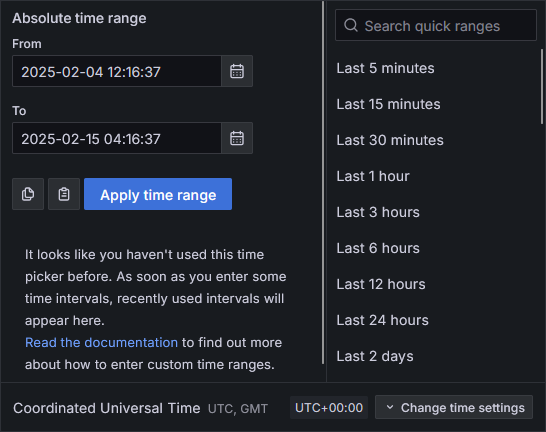
\includegraphics[width=0.6\textwidth, keepaspectratio]{images/timerange.png}
    \caption{Grafana Time Picker}
    \label{fig:timerange}
\end{figure}

Neben der Filterung nach Zeiträumen ermöglicht Grafana die Definition von Variablen, die in den Einstellungen erstellt und je nach Konfiguration auf dem Dashboard angezeigt werden. Diese Variablen dienen als Platzhalter in SQL-Queries oder API-Abfragen. Wählt der Nutzer einen Variablenwert aus, werden alle Panels, die diese Variable enthalten, dynamisch angepasst und zeigen die entsprechend gefilterten Daten an. \parencite{GrafanaLabsVariables}

\subsection{Sicherheit und Zugriffskontrolle}
Um den Zugriff auf das Dashboard zu schützen, stellt Grafana standardmäßig eine integrierte Authentifizierungsfunktion bereit. Bei der ersten Anmeldung wird ein vordefiniertes Admin-Konto mit dem Benutzernamen \verb|admin| und einem Standardpasswort eingerichtet. Aus Sicherheitsgründen sollte dieses Passwort unmittelbar nach dem ersten Login geändert werden. Außerdem liefert Grafana ein rollenbasiertes Zugriffssystem. In der Open Source Version stehen die drei vordefinierten Rollen Viewer, Editor und Admin zur Verfügung. Viewer können Dashboards nur anzeigen, während Editoren zusätzlich Dashboards bearbeiten und neue Panels erstellen dürfen. Administratoren haben vollständigen Zugriff auf alle Konfigurationen innerhalb der Grafana-Instanz. Eine erweiterte rollenbasierte Zugriffskontrolle, die eine feingranulare Berechtigungsverwaltung für Benutzergruppen und API-Zugriffe ermöglicht, ist nur in Grafana Enterprise und Grafana Cloud verfügbar. \parencite{GrafanaRBAC}

Für eine verschlüsselte Verbindung über HTTPS muss in Grafana nichts weiter konfiguriert werden, da hierfür ein Reverse Proxy für die Weiterleitung an Grafana verwendet wird.

\section{Responsive Design}
\label{sec:responsive-design}
Grafana verwendet ein Grid-Layout für die Anordnung der Panels. Diese können auf der Nutzeroberfläche durch den Administrator beliebig in diesem Gitter verschoben werden. Ebenfalls wird standardmäßig der Wert \verb|auto| für die Breite (engl. width) der Panels gesetzt, sodass sich diese automatisch an die Bildschirmgröße des Nutzers anpasst.
    \chapter{Implementierung}
\label{ch:implementierung}

\section{Netzwerk- und Speicherstruktur der Container-Umgebung}
Die gesamte Umgebung wird durch eine \texttt{docker-compose.yml} orchestriert. Orchestrierung bedeutet die automatische Vernetzung und Verwaltung der erstellten Container, sodass diese als zusammenhängendes System funktionieren \parencite{AWS}. In der \texttt{docker-compose.yml} wird das interne Netzwerk \texttt{matomo\textunderscore network} erstellt, über welches die Container miteinander kommunizieren. Zusätzlich werden persistente Volumes definiert, um sicherzustellen, dass die Daten über Neustarts der Container hinweg erhalten bleiben. Das Volume \texttt{matomo} speichert sämtliche Konfigurationsdateien des Webanalyse-Tools. Somit können die Matomo Einstellungen, beispielsweise für den Datenschutz persistent gespeichert werden. Die Datenbank, welche alle erfassten Trackingdaten enthält wird in dem Volume \texttt{db} gespeichert. Für die Visualisierung speichert das Volume \texttt{grafana-storage} die Konfigurationen von Grafana, sowie die erstellten Dashboards und Panels. Das Bildungsportal wird als externes Volume \texttt{portal} aus dem Projektverzeichnis eingebunden.

\section{Reverse Proxy und Dienstweiterleitung}
Der Reverse Proxy (Nginx) wird als Zugangspunkt für die Dienste verwendet. Die Konfigurationsdatei \texttt{reverse\textunderscore proxy.conf} dient dazu, die externen Anfragen an die Dienste weiterzuleiten. Somit werden die Website, Matomo und Grafana unter separaten Pfaden erreichbar gemacht: 

\textbf{Matomo} wird über den Reverse Proxy unter \texttt{/matomo} bereitgestellt. Da das verwendete Matomo-Docker-Image \texttt{/matomo:5.2.2-fpm-alpine} keinen eigenen Webserver mitbringt, wird in der \texttt{docker-compose.yml} ein zusätzlicher Nginx-Webserver (\texttt{matomo\textunderscore web}) definiert. Dieser empfängt Anfragen vom Reverse Proxy und leitet sie über das FastCGI-Protokoll an PHP-FPM (FastCGI Process Manager) weiter, da Matomo auf PHP basiert. PHP-FPM ist ein Prozessmanager für PHP \parencite{PHPFPM}, welcher von Matomo verwendet wird. Da Nginx als Reverse Proxy keine PHP-Skripte selbst verarbeiten kann, sondern diese an eine externe Instanz übergeben muss \parencite{NginxReverseProxy}, ist dieser zusätzliche Webserver erforderlich. Dieser benötigt ebenfalls eine Konfig-Datei (\texttt{matomo.conf}), die sicherstellt, dass alle Anfragen korrekt verarbeitet und an PHP-FPM übergeben werden. Während die \texttt{reverse\textunderscore proxy.conf} externe Anfragen an \texttt{/matomo} an \texttt{matomo\textunderscore web} weiterleitet, definiert die \texttt{matomo.conf}, wie diese innerhalb des Containers verarbeitet werden. Der \texttt{matomo\textunderscore web}-Container besitzt kein öffentliches Port-Mapping und ist ausschließlich über den Reverse Proxy erreichbar.

\textbf{Grafana} wird unter \texttt{/grafana} bereitgestellt. Im Gegensatz zu Matomo benötigt Grafana keinen separaten Webserver, da es über einen integrierten Webserver verfügt. Dadurch kann Grafana direkt über den Reverse Proxy erreichbar gemacht werden.

\textbf{Die Website} wird unter \texttt{/evaschiffmann} bereitgestellt. Sie wird ebenfalls wie Matomo über einen Nginx-Webserver ausgeliefert, der ausschließlich für die Bereitstellung der Inhalte zuständig ist. Genauso wie \texttt{matomo\textunderscore web} besitzt auch dieser Webserver kein öffentliches Port-Mapping, sodass die Website nur über den Reverse Proxy aufgerufen werden kann. Dieser nimmt die Anfragen entgegen und leitet sie an den internen Nginx-Container weiter, welcher die Website ausliefert.

\begin{figure}[H]
    \centering
    \begin{minipage}{\textwidth}
        \lstinputlisting[
            caption=Docker Container zur Bereitstellung des Nginx Reverse Proxy, 
            label={lst:reverseproxy},
            language={}, 
            style=yaml
        ]{listings/reverse-proxy.yml}
    \end{minipage}
\end{figure}

Das Listing~\ref{lst:reverseproxy} zeigt die Definition des Reverse Proxy in der \texttt{docker-compose.yml}. Die einzelnen Komponenten werden anhand der Kommentare beschrieben. Um die Dienste über HTTPS verfügbar zu machen, wurde für die Testumgebung auf localhost ein selbst signiertes Zertifikat erstellt und eingebunden. Dies ist in Zeile 8 zu erkennen. In Zeile 10 wird das Volume für Matomo gemountet, sprich eingebunden. Dies dient zur Bereitstellung von statischen Inhalten wie HTML oder Javascript. PHP-Anfragen werden, wie bereits erwähnt, an \texttt{matomo\textunderscore web} weitergeleitet.

\section{Integration der Webanalyse mit Matomo}
Nachdem die Webserver aufgesetzt wurden und die \texttt{docker-compose.yml} definiert wurde, ist Matomo in der lokalen Umgebung über \textit{https://localhost/matomo} verfügbar und die Einrichtung kann erfolgen. Die Einrichtung besteht im wesentlichen aus fünf Schritten. Zunächst wird ein System Check durchgeführt, bei dem überprüft wird, ob die Serverumgebung die Anforderungen für den Betrieb von Matomo erfüllt. Hierbei wird unter anderem geprüft, ob eine kompatible PHP-Version verwendet wird oder auch ob Matomo auf die notwendigen Verzeichnisse zugreifen kann und Schreibrechte für diese besitzt. Nach dem erfolgreichen System Check kann die Datenbankverbindung eingerichtet und ein Hauptadministrator angelegt werden. 

\begin{figure}[H]
    \centering
    \begin{minipage}{0.49\textwidth}
        \centering
        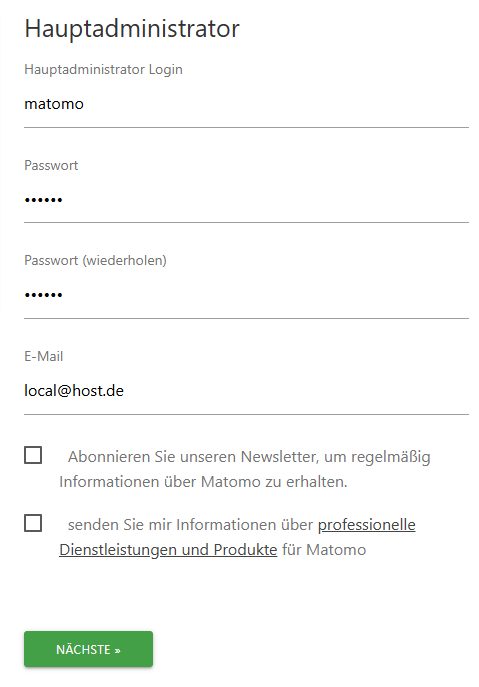
\includegraphics[width=\linewidth, keepaspectratio]{images/haupadministrator.png}
        \caption{Anlegen des Kontos für den Hauptadministrator in Matomo}
        \label{fig:hauptadministrator}
    \end{minipage}
    \hfill
    \begin{minipage}{0.49\textwidth}
        \centering
        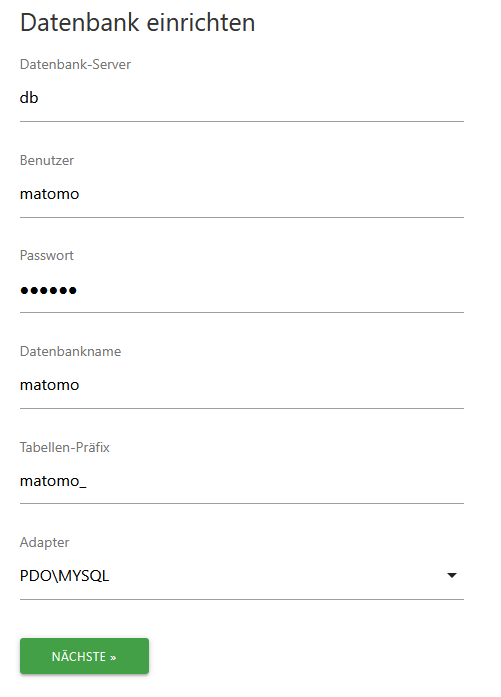
\includegraphics[width=\linewidth, keepaspectratio]{images/setup-datenbank.png}
        \caption{Einrichtung der Datenbankverbindung in Matomo}
        \label{fig:setup-datenbank}
    \end{minipage}
\end{figure}

In Abbildung~\ref{fig:hauptadministrator} ist zu sehen, wie das Konto erstellt wird. In Abbildung~\ref{fig:setup-datenbank} wird gezeigt, wie die Datenbankverbindung zu MariaDB hergestellt wird. Die Zugangsdaten für den Hauptadministrator sowie den Datenbanknutzer sind in der Datei \texttt{db.env} gespeichert. Für die Datenbank wird der Container \texttt{db} verwendet. In diesem Container wird dafür gesorgt, dass folgendes Skript eingebunden wird: 

\begin{figure}[H]
    \centering
    \begin{minipage}{\textwidth}
        \lstinputlisting[
            caption=SQL-Skript für die Erstellung eines Nutzer mit read-only Rechten, 
            label={lst:readonly},
            language=sql
        ]{listings/create-read-only-user.sql}
    \end{minipage}
\end{figure}

Das in Listing~\ref{lst:readonly} zu sehende Skript erstellt einen neuen Datenbanknutzer, welcher ausschließlich Leseberechtigung auf die Datenbanktabellen von Matomo besitzt. Dieser Datenbanknutzer soll später für die Anbindung an Grafana verwendet werden, um sicherzustellen, dass über Grafana keine Daten manipuliert werden können. 

Im vorletzten Schritt der Einrichtung wird die Website konfiguriert, welche von Matomo getrackt werden soll. Die Website erhält einen Namen in Matomo, worüber direkt erkannt werden kann, welche Website getrackt wird. Ebenfalls muss in diesem Schritt die URL des Bildungsportals angegeben werden, damit das Tracking auf diesem erfolgen kann.  

Im letzten Schritt der Matomo-Einrichtung wird das Page-Tag von Matomo generiert. Um dieses nutzbar zu machen, wird es anschließend vor dem \texttt{</body>}-Tag jeder Seite integriert, um sicherzustellen, dass der Inhalt der Seite geladen wurde. Da die gespiegelte Website sehr viele HTML-Dateien beinhaltet, wurde hierfür ein Python-Skript (\texttt{insert\allowbreak-scripts.py}) geschrieben, welches dafür sorgt, dass das Page-Tag in alle HTML-Dateien per Skript-Tag eingefügt wird. Die Datei \texttt{tracking.js} enthält das eigentliche Page-Tag sowie alle notwendigen Tracking-Events.


\section{Matomo datenschutzkonform konfigurieren}
Damit sichergestellt wird, dass Nutzer nicht über ihre IP-Adressen identifiziert werden können, wird in Matomo innerhalb der Einstellungen zur Privatsphäre eine IP-Anonoymisierung konfiguriert. Hierbei werden die letzten zwei Bytes der IP-Adresse anonymisiert. Um den Nutzer darüber zu informieren, welche Daten erfasst und zu welchem Zweck diese verarbeitet werden, befindet sich auf der Datenschutzseite des Bildungsportals bereits ein entsprechender Hinweistext.

Um sicherzustellen, dass Nutzer nur dann getrackt werden, wenn diese ihre Zustimmung erteilen, werden Opt-In- und Opt-Out-Mechanismen für die Einwilligung und den Widerruf der Tracking-Berechtigungen implementiert. Hierfür wurde im Page-Tag die in Listing~\ref{lst:require-consent} zu sehende Zeile hinzugefügt: 

\begin{figure}[H]
    \centering
    \begin{minipage}{\textwidth}
        \lstinputlisting[
            caption=Funktion zur Überprüfung der Nutzereinwilligung für das Tracking in Matomo, 
            label={lst:require-consent},
        ]{listings/require-consent.js}
    \end{minipage}
\end{figure}

Hierdurch verhindert Matomo, dass Tracking-Daten automatisch erfasst werden, solange keine Einwilligung vorliegt. Erst wenn der Nutzer aktiv zustimmt, wird das Tracking aktiviert \parencite{MatomoConsent}.

Die Zustimmung, also das Opt-In, erfolgt über das Cookie-Banner. Wenn hierbei auf \glqq Ok\grqq{} geklickt wird, wird der in Listing~\ref{lst:remember-consent-given} zu sehende Programmcode ausgeführt:

\begin{figure}[H]
    \centering
    \begin{minipage}{\textwidth}
        \lstinputlisting[
            caption=Programmcode zum Setzen der Zustimmung für das Tracking in Matomo, 
            label={lst:remember-consent-given},
        ]{listings/remember-consent-given.js}
    \end{minipage}
\end{figure}

Sobald hierbei der Klick auf \glqq Ok\grqq{} erfolgt ist, wird die Funktion \texttt{rememberConsentGiven} ausgeführt. Diese Funktion sorgt dafür, dass ein Cookie Namens \glqq consent\grqq{} im Browser des Nutzers gesetzt wird \parencite{MatomoConsent}. So lange dieser Cookie existiert hat Matomo die Erlaubnis Daten zu sammeln \parencite{MatomoConsent}. Zusätzlich wird der Einwilligungsstatus im lokalen Speicher des Browsers (\texttt{localStorage}) gespeichert.

Die Speicherung zusätzlich im lokalen Speicher des Browsers ist notwendig, da dieser Status in der Datei \texttt{withdraw-consent.js} verwendet wird. Die Logik dieser Datei ist in Listing~\ref{lst:withdraw-consent} zu erkennen: 

\begin{figure}[H]
    \centering
    \begin{minipage}{\textwidth}
        \lstinputlisting[
            caption=Programmcode zur Speicherung und Verwaltung der Tracking-Einwilligung mittels Local Storage,
            label={lst:withdraw-consent},
        ]{listings/withdraw-consent.js}
    \end{minipage}
\end{figure}

In Zeile 2 wird als erstes geprüft, ob der Consent für das Tracking erteilt wurde. Auf der Datenschutzseite wurde ein Button für das Widerufen und die Zustimmung zum Tracking hinzugefügt. In den Zeilen 7 bis 10 wird der Button-Text entsprechend des aktuellen Tracking-Status gesetzt. Ist das Tracking bereits aktiv, wird der Text \glqq Tracking deaktivieren\grqq{} angezeigt, andernfalls erscheint \glqq Tracking erlauben\grqq{}. Die Zeilen 14 bis 28 enhalten die Logik um die Zustimmung oder Ablehnung den Trackings zu setzen. Hierbei wird jeweils eine Meldung an den Nutzer gegeben, dass die Aktion erfolgreich war. Im lokalen Speicher des Browsers wird ebenfalls der Status zur Zustimmung gespeichert. Die Zustimmung über den Button erfolgt ebenfalls wie bei dem Cookie-Banner über \texttt{rememberConsentGiven}. Für das Widerrufen der Berechtigung wird die Funktion \texttt{forgetConsentGiven} verwendet, welche dafür sorgt, dass der gesetzte \glqq consent\grqq{}-Cookie gelöscht wird \parencite{MatomoConsent}.

\section{Einrichtung der Datenquelle in Grafana}
Grafana ist in der lokalen Umgebung unter \textit{https://localhost/grafana} verfügbar. Wird diese URL aufgerufen, erscheint zunächst der Login-Screen zur Anmeldung. Nach erfolgter Anmeldung wird die Grafana Oberfläche geladen. Um nun Analysedaten von Matomo zu erhalten, muss zunächst eine Datenquelle eingerichtet werden. Da direkt auf Daten aus der Matomo Datenbank zugegriffen werden soll, wird hierfür die Grafana Datenquelle \glqq MySQL\grqq{} verwendet.

\begin{figure}[H]
    \centering
    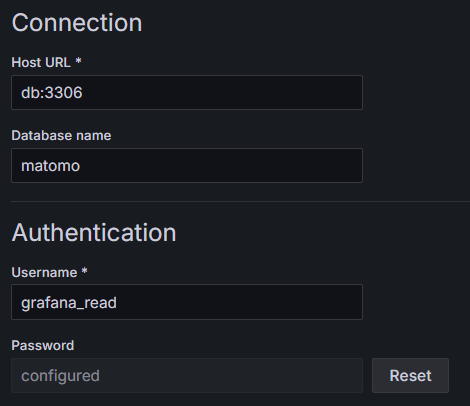
\includegraphics[width=0.6\textwidth, keepaspectratio]{images/datasource.png}
    \caption{Einrichtung der Datenquelle in Grafana über das MySQL-Plugin}
    \label{fig:datasource}
\end{figure}

In der Abbildung~\ref{fig:datasource} ist zu sehen, dass der Datenbank-Container \texttt{db} mit dem Standardport für MySQL bzw. MariaDB als Host URL gesetzt wurde. Dies ist möglich, da Grafana und Matomo über das gemeinsame Netzwerk \texttt{matomo\textunderscore network} innerhalb der Container-Umgebung kommunizieren können. Somit kann direkt der Containername, anstatt einer URL verwendet werden. Ebenfalls zu erkennen ist, dass der zuvor erstellte Datenbanknutzer, welcher ausschließlich Leseberechtigungen auf die Matomo Datenbank besitzt, verwendet wird, um Daten abzurufen. Wenn nun Panels zur Visualisierung der Analysewerte erstellt werden, kann diese Datenquelle ausgewählt werden, um über den read-only Nutzer der Datenbank SQL-Abfragen an diese zu erstellen.

\section{Umsetzung der Filtermöglichkeiten in Grafana}
Um die zeitliche Filterung der erhaltenen Daten einheitlich über alle Pannels hinweg zu ermöglichen, wird der Grafana Time Picker verwendet. Damit dieser funktionsfähig ist, müssen die über den Time Picker eingestellten Werte in die SQL-Abfrage integriert werden. Hierfür werden die Grafana-Variablen \texttt{\$\{\_\_from\}} und \texttt{\$\{\_\_to\}} genutzt, welche das Start- und Enddatum der vom Nutzer gewählten Zeitspanne enthalten \parencite{GrafanaTimePickerVariables}. 

\begin{figure}[H]
    \centering
    \begin{minipage}{\textwidth}
        \lstinputlisting[
            caption=Zeitliche Filterung der Besuchsdaten in Grafana über die Variablen \texttt{\$\{\_\_from\}} und \texttt{\$\{\_\_to\}},
            label={lst:from-to},
            language=sql
        ]{listings/from-to.sql}
    \end{minipage}
\end{figure}

In dem Listing~\ref{lst:from-to} werden die Grafana Variablen für die Zeitbegrenzung verwendet. Da der Time Picker nur Unix Zeitstempel zurückgibt, müssen diese in das passende Datumsformat der Datenbank umgewandelt werden. Hierfür bietet MySQL die Funktion \texttt{FROM\textunderscore UNIXTIME} \parencite{MySQLUnixtime}. Die Tabelle \texttt{log\textunderscore visit} wird für die Zeitbegrenzung verwendet und speichert die einzelnen Nutzersitzungen \parencite{MatomoDBSchema}. In dieser Tabelle befindet sich die Spalte \texttt{visit\textunderscore first \textunderscore action\textunderscore time}, welche den Zeitpunkt der ersten Aktion einer Sitzung speichert \parencite{MatomoDBSchema}. Da jeder Eintrag eine eigenständige Sitzung darstellt, können darüber Sitzungen gefiltert werden, die im gewählten Zeitraum stattgefunden haben.

Um die Filterung der Werte für die einzelnen Unterseiten zu realisieren, wird in Grafana die Variable \texttt{\$Seite} definiert. Diese hat als Werte die Titel der Unterseiten des Bildungsportals, also beispielsweise \glqq Zum Tagebuch\grqq{} oder \glqq Schülerin\grqq{}. Die Variable kann ebenfalls den Wert \glqq Übersicht\grqq{} haben. Wenn dieser Wert ausgewählt wird, werden die angezeigten Daten nicht auf eine bestimmte Unterseite begrenzt, sondern beziehen sich auf das gesamte Bildungsportal. Ebenso kann für die Variable der Wert \glqq Alle Tagebuchseiten\grqq{} ausgewählt werden. Hierbei werden alle Tagebuchseiten zusammengefasst, um eine Übersicht über die allgemeine Nutzung des Tagebuchs zu zeigen. Nachdem die Variable definiert wurde, wird diese in der Dashboardansicht sichtbar und über ein Drop-Down Menü können die einzelnen Werte der Variable ausgewählt werden.

\begin{figure}[H]
    \centering
    \begin{minipage}{\textwidth}
        \lstinputlisting[
            caption=SQL-Abfrage zur Filterung der Besuche basierend auf der ausgewählten Unterseite oder den Tagebuchseiten,
            label={lst:seite},
            language=sql
        ]{listings/seite.sql}
    \end{minipage}
\end{figure}

Das Listing~\ref{lst:seite} zeigt, auf welche Art und Weise die Variable \texttt{\$Seite} in den SQL-Abfragen verwendet wird. Über diese Query werden alle Besuche auf der Website ausgegeben, entweder ungefiltert, für eine Unterseite oder für alle Tagebuchseiten. Über den ersten \texttt{JOIN} in Zeile 5 werden die Sitzungen mit den zugehörigen Aktionen, also unter anderem Seitenaufrufen, verknüpft. Da die Seitentitel allerdings in der Tabelle \texttt{log\textunderscore action} gespeichert werden, wird hierfür ein weiterer \texttt{JOIN} benötigt. In der {\texttt{WHERE}-Klausel} wird zuletzt der Wert der Variable geprüft. Ist dieser \glqq Übersicht\grqq{} wird keine Filterung vorgenommen und alle Besuche werden angezeigt. Wird eine Unterseite ausgewählt, werden nur die Besuche auf dieser Seite ausgegeben. Für die Tagebuchseiten wurde ein regulärer Ausdruck verwendet, da die Titel für die Tagebuchseiten immer den Bezeichner \glqq Blatt\grqq{} mit der entsprechenden Nummer besitzen.

Die Variable \texttt{\$Seite} wird in diesen Metriken verwendet: 
\begin{itemize}
    \item Anzahl der Besuche
    \item Anzahl der wiederkehrenden Besucher
    \item Anteil der wiederkehrenden Besucher
    \item Anzahl der einmaligen Besucher
    \item Ranking der am häufigsten aufgeklappten Überschriften
    \item Verweildauer
\end{itemize}

Um die Sortierrichtung der Tabellen sowie des Balkendiagramms umzukehren, wird eine Variable namens \texttt{\$Sort} definiert. Diese Variable hat die Werte \textit{ASC} (aufsteigend) und \textit{DESC} (absteigend).

\begin{figure}[H]
    \centering
    \begin{minipage}{\textwidth}
        \lstinputlisting[
            caption=SQL-Abfrage zur Identifikation von Traffic-Quellen sowie zur Erfassung der Seitenaufrufe und Absprungraten über diese,
            label={lst:referer-ranking},
            language=sql
        ]{listings/referer-ranking.sql}
    \end{minipage}
\end{figure}

Die Query aus Listing~\ref{lst:referer-ranking} zeigt, wie die Variable \texttt{\$Sort} verwendet wird. Je nach Auswahl wird der Wert in die {\texttt{ORDER BY}-Klausel} geschrieben. Der \texttt{referer\textunderscore type} wird in der Datenbank als Zahlenwert gespeichert, wobei jede Zahl einen Quelle angibt \parencite{MatomoDBSchema}. Wenn der Zugriff nicht über einen Referer erfolgt, ist der \texttt{referer\textunderscore type} gleich \glqq 1\grqq{}. Dieser Wert wird somit ausgeschlossen. Matomo speichert in der Datenbank ebenfalls die Aktionen, welche auf der Website ausgeführt wurden, nachdem der Besucher über einen Referer auf die Seite gelangt ist. Wenn nur eine Aktion ausgeführt wurde, so wird der \texttt{bounce\textunderscore count} gesetzt. Dieser Zähler erhöht sich um eins, wenn Besucher nur eine Aktion ausführen, wenn diese über eine externe Quelle auf das Bildungsportal gelangt sind. Die Gruppierung erfolgt über die \texttt{referer\textunderscore url}, sodass die Besuche und Absprünge für jede URL angezeigt werden. 

Die Variable \texttt{\$Sort} wird in diesen Metriken verwendet: 
\begin{itemize}
    \item Ranking der Referer Seiten
    \item Seitenaufrufe nach Häufigkeit
    \item Ranking der am häufigsten aufgeklappten Überschriften
\end{itemize}

\section{Erstellung der Panels in Grafana}
In diesem Abschnitt wird beschrieben, wie sich die einzelnen Abfragen zu den Analysewerten zusammensetzen und wie die Panels für die Visualisierung konfiguriert werden, um die in Abschnitt~\ref{sec:Visualisierungsmethoden} beschriebenen Visualisierungsformen für die entsprechenden Analysewerte zu verwenden. Jedes Panel verfügt über einen eindeutigen Titel und eine Beschreibung, welche den dargestellten Analysewert erläutert.

\subsection{Ranking der Referer Seiten}
Die Abfrage für diese Metrik ist in Listing~\ref{lst:referer-ranking} zu sehen und wurde bereits erklärt. In den Panel-Einstellungen wird als Darstellungsform die Tabelle ausgewählt. Über die Einstellung \glqq Show table header\grqq{} wird eingestellt, dass die in der SQL-Abfrage definierten Namen für die Tabellen im Panel angezeigt werden. Außerdem wird für die Größe der Tabelle die \glqq Cell Height\grqq{}
(Zeilenhöhe) auf \glqq Medium\grqq{} gesetzt. Eine kleinere Zeilenhöhe würde die Übersichtlichkeit beeinträchtigen, während eine größere dazu führen würde, dass weniger Werte auf einen Blick erfassbar sind. Der Hintergrund für die Spalten \texttt{Besuche} und \texttt{Bounce\textunderscore Count} wird mit dem Lila-Farbton des Bildungsportals versehen, während die Spalte \texttt{Referer} den Gelbton des Bildungsportals erhält.

\subsection{Verteilung der Traffic Quellen}
Für die Verteilung der Traffic Quellen wird in Grafana ein Pie-Chart-Panel erstellt, um die Daten in einem Kreisdiagramm zu visualisieren. Hierbei ist es wichtig, dass die Einstellung \texttt{Show} auf \glqq All values\grqq{} gesetzt wird. Andernfalls würde die Gesamtzahl der Traffic-Quellen angezeigt werden. Grafana bietet die Darstellungsformen \texttt{Pie} und \texttt{Donut} für das Pie-Chart-Panel. Hierbei bietet die \texttt{Pie}-Option die größere Fläche für die Darstellung der Prozentwerte, weshalb diese Option verwendet wird. Ein Tooltip wird integriert, der beim Überfahren der einzelnen Bereiche des Kreisdiagramms mit der Maus den jeweiligen Prozentwert anzeigt. Ebenfalls gibt es eine Legende, welche die einzelnen Werte mit den entsprechenden Farben sowie Prozentwerten darstellt.

Für die Datenbankabfrage wird die Tabelle \texttt{log\textunderscore visit} verwendet, in welcher die Referer-Informationen gespeichert werden. Die in Lisiting~\ref{lst:referer-ranking} aufgezeigten \texttt{referer\textunderscore types}, kommen für diese Metrik ebenfalls zum Einsatz. Zusätzlich wird der Wert \glqq 1\grqq{} mit aufgenommen, um den Prozentsatz der Nutzer, welche direkt auf die Website über die Eingabe der URL oder auch über ein Lesezeichen gelangt sind, zu berücksichtigen. Damit im Kreisdiagramm die richtigen Werte für die verschiedenen Quellen angezeigt werden, müssen diese entsprechend dem \texttt{referer\textunderscore type} gruppiert werden.

\subsection{Seitenaufrufe nach Häufigkeit}
Für diese Metriken wird ein Bar-Chart-Panel verwendet. Hierfür bietet Grafana umfangreiche Konfigurationsmöglichkeiten: 

\begin{figure}[H]
    \centering
    \begin{minipage}{0.49\textwidth}
        \centering
        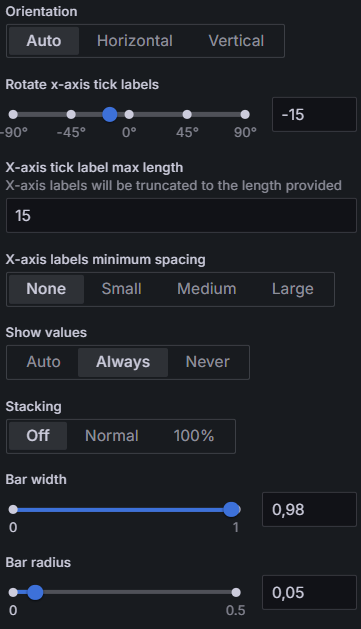
\includegraphics[width=\linewidth, keepaspectratio]{images/orientation.png}
        \caption{Anpassung der Balkendiagramm-Ausrichtung, Balkenbreite und Beschriftungen in Grafana}
        \label{fig:orientation}
    \end{minipage}
    \hfill
    \begin{minipage}{0.49\textwidth}
        \centering
        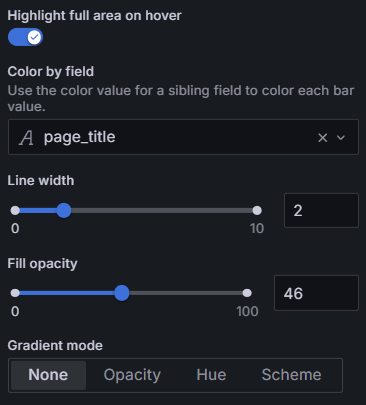
\includegraphics[width=\linewidth, keepaspectratio]{images/highlight.png}
        \caption{Einstellungen zur Hervorhebung und Farbgebung im Balkendiagramm in Grafana}
        \label{fig:highlight}
    \end{minipage}
\end{figure}

Wie in Abbildung~\ref{fig:orientation} zu sehen ist, wird der Winkel der X-Achsen-Beschriftungen leicht angepasst, um die Lesbarkeit der Seitentitel zu verbessern und ein Überlappen der Texte zu vermeiden. Zusätzlich wird die maximale Zeichenlänge der X-Achsen-Beschriftungen auf \glqq 15\grqq{} begrenzt, sodass lange Titel gekürzt werden. Die Ausrichtung des Diagramms kann zwischen horizontal und vertikal gewechselt werden, wobei die aktuelle Einstellung \glqq Auto\grqq{} einer horizontalen Darstellung entspricht. Zudem wird die Balkenbreite und der Balkenradius angepasst, um ein abgerundetes Design zu erzeugen. Durch die aktivierte Option \texttt{Show values} wird sichergestellt, dass die Zahlenwerte direkt auf den Balken angezeigt werden, ohne das diese nochmal separat angeklickt werden müssen.

In Abbildung~\ref{fig:highlight} sind die Einstellungen für die optische Darstellung der Balken zu sehen. Hier wird festgelegt, dass beim Überfahren eines Balkens mit der Maus der gesamte Bereich farblich markiert wird. Die Farbgebung der Balken richtet sich nach dem Feld \texttt{page\textunderscore title}, um eine visuelle Unterscheidung zwischen den einzelnen Seitentiteln zu ermöglichen. Unterseiten erhalten jeweils eine eigene Farbe, wobei für alle Tagebuchseiten die selbe Farbe verwendet wird. Das ist ebenfalls der Fall für die Unterseiten von \glqq Wer war Eva Schiffmann\grqq{} und \glqq Themen\grqq{}. Diese Entscheidung wurde getroffen, da ansonsten mit verschiedenen Farbtönen einer Farbe gearbeitet werden müsste und somit die Unterscheidung zwischen den Seiten schwerer fällt. Darüber hinaus wird die Linienbreite reduziert und die Transparenz der Balkenfüllung angepasst, um das Diagramm optisch ansprechender zu machen.

\begin{figure}[H]
    \centering
    \begin{minipage}{\textwidth}
        \lstinputlisting[
            caption=SQL-Abfrage für die Metrik \glqq Seitenaufrufe nach Häufigkeit\grqq{},
            label={lst:seitenaufrufe},
            language=sql
        ]{listings/seitenaufrufe.sql}
    \end{minipage}
\end{figure}

Das Listing~\ref{lst:seitenaufrufe} zeigt die SQL-Abfrage zur Ermittlung der zehn meist- oder wenigstbesuchten Unterseiten. Über einen \texttt{JOIN} wird die Tabelle \texttt{log\textunderscore link\textunderscore visit\textunderscore action} mit \texttt{log\textunderscore action} verknüpft, um die zugehörigen Seitentitel abzurufen. Ein weiterer \texttt{JOIN} mit der Tabelle \texttt{log\textunderscore visit} verknüpft die Aktionen mit den jeweiligen Besuchssitzungen.

Zusätzlich wird über eine \texttt{CASE}-Anweisung geprüft, ob es sich bei einer Seite um eine Tagebuchseite handelt. In diesem Fall wird mithilfe eines regulären Ausdrucks der Titel standardisiert, sodass alle Tagebuchseiten unter einer gemeinsamen Bezeichnung zusammengefasst werden. Die Abfrage zählt die Seitenaufrufe, sortiert sie nach Häufigkeit und gibt die zehn meist- oder wenigstbesuchten Seiten zurück.

\subsection{Ranking der am häufigsten aufgeklappten Überschriften}
Diese Metrik verwendet ebenfalls eine Tabelle für die Visualisierung. Wie bei der Tabelle \glqq Ranking der Referer Seiten\grqq{} werden die Farben des Bildungsportals für die Hintergründe der Spalten gesetzt. Die Spalte \glqq Anzahl\grqq{} hat den Lila-Farbton und der Hintergrund der Spalte \glqq Titel\grqq{} ist gelb. Der \glqq Titel\grqq{} gibt an, um welche Überschrift es sich handelt und die \glqq Anzahl\grqq{} zeigt, wie oft die Überschrift aufgeklappt wurde. Die Panel-Einstellungen werden ebenfalls identisch zur Metrik \glqq Ranking der Referer Seiten\grqq{} gesetzt, um für ein einheitliches Design zu sorgen. Da für das Aufklappen der Überschriften kein Page-View getriggert wird, muss um diese Metrik zu erfassen, ein Event definiert werden. Dieses wird in Listing~\ref{lst:headingsevent} dargestellt:

\begin{figure}[H]
    \centering
    \begin{minipage}{\textwidth}
        \lstinputlisting[
            caption=Matomo-Events für die Erfassung der Interaktionen mit den Überschriften.,
            label={lst:headingsevent},
        ]{listings/headings-event.js}
    \end{minipage}
\end{figure}

In diesem Programmcode werden Events gesendet, sobald mit einer Überschrift auf der Website interagiert wird. Neben dem Event für das Aufklappen der Überschriften wird noch ein Event für das Zuklappen benötigt. Die Differenz zwischen dem Aufklappen und Zuklappen wird genutzt, um zu bestimmen, wie lange der Text gelesen wurde. Die Kategorie des Events \texttt{expand} enhält außerdem den Titel der Überschrift. Für das \texttt{close}-Event wird der Titel nicht benötigt, da sich dieses immer auf die zuvor aufgeklappte Überschrift bezieht. Dies ist möglich, da Überschriften auf der Website automatisch zugeklappt werden, wenn eine weitere Überschrift aufgeklappt wird. Das Event \texttt{close} wird für diese Metrik zwar nicht benötigt, spielt aber für die Analyse einer Nutzersitzung eine Rolle.

Die Abfrage zu diesem Panel verwendet für die Events die Tabelle \texttt{log\textunderscore action}. Da für das \glqq Ranking der am häufigsten aufgeklappten Überschriften\grqq{} nur das Event \texttt{expand} berücksichtigt wird, wird \texttt{log\textunderscore action} mehrfach per Self-Join eingebunden. Das ist notwendig, da Matomo Kategorie, Aktion und Label eines Events gemeinsam in dieser Tabelle speichert. Um alle drei Bestandteile getrennt auswerten zu können, muss die Tabelle mit unterschiedlichen Aliasen gejoint werden. Nur so lässt sich beispielsweise der Titel (Label) mit der Aktion \texttt{expand} korrekt verknüpfen. Die Tagebuchseiten enthalten ebenfalls jeweils drei Überschriften, welche für jede Seite gleich sind. Damit diese Überschriften in dem Panel ignoriert werden, wird die in Listing~\ref{lst:ignorieren} zu sehende Zeile in der Query ergänzt: 

\begin{figure}[H]
    \centering
    \begin{minipage}{\textwidth}
        \lstinputlisting[
            caption=Ausschnitt einer SQL-Abfrage\, um die Überschriften innerhalb der Tagebuchseiten zu ignorieren,
            label={lst:ignorieren},
            language=sql
        ]{listings/ignore.sql}
    \end{minipage}
\end{figure}

\texttt{event\textunderscore label} ist ein Alias für die Tabelle \texttt{log\textunderscore action} und über das Attribut \texttt{name} wird der Titel der Überschrift gefiltert.

\subsection{Besuche, einmalige Besucher und wiederkehrende Besucher}
Zur Darstellung dieser drei Metriken wird ein einfaches statisches Panel verwendet und der Hintergrund wird auf den Gelbton des Bildungsportal gesetzt.

Die Abfrage für die Besuche ermittelt die Gesamtanzahl der Nutzer, die eine Seite des Bildungsportals besucht haben. Dafür wird die Tabelle \texttt{log\textunderscore action} mit \texttt{log\allowbreak\_link\allowbreak\_visit\allowbreak\_action} verknüpft. Die Anzahl der unterschiedlichen Visit-ID's in der Tabelle \texttt{log\textunderscore action} entspricht hierbei der Anzahl der Besuche. Die Abfrage für diese Metrik ist in Listing~\ref{lst:seite} dargestellt und wurde bereits im Zusammenhang mit der Erklärung der Variable \texttt{\$Seite} erläutert.

Die Query für die wiederkehrenden Besucher basiert auf derselben Tabellenstruktur, konzentriert sich aber auf Nutzer, welche die Website bereits zuvor besucht haben. Dazu wird \texttt{visitor\textunderscore returning = 1} als Bedingung gesetzt. Der Wert \glqq 1\grqq{} gibt an, dass der Besucher bereits zuvor auf der Website war. Die Zählung erfolgt, anders als bei der Metrik für die Besuche, über die Visitor-ID. Der Unterschied hierbei ist, dass nicht einzelne Sitzungen (Besuche) gezählt werden, sondern tatsächliche Besucher.

Die Metrik für die einmaligen Besucher identifiziert Nutzer, die exakt eine Session auf der Website hatten. Über eine Unterquery wird geprüft, welche Visitor-ID's nur genau einmal in der \texttt{log\textunderscore action}-Tabelle vorkommen, also nur eine einzelne Sitzung aufweisen. Das geschieht über die Filterung \texttt{HAVING COUNT(idvisit) = 1}. Die Seitenfilterung erfolgt auch hierbei genauso wie für die Besuche.

\subsection{Anteil der wiederkehrenden Besucher}
Der \glqq Anteil der wiederkehrenden Besucher\grqq{} wird über ein Gauge-Panel realisiert. Der Wert erhält außerdem die Maßeinheit \%. Es werden drei Grenzwerte (engl. Thresholds) definiert, um dabei zu helfen, den angezeigten Wert auf den ersten Blick einzuordnen. Die Thresholds sind in Abbildung~\ref{fig:thresholds} zu sehen: 

\begin{figure}[H]
    \centering
    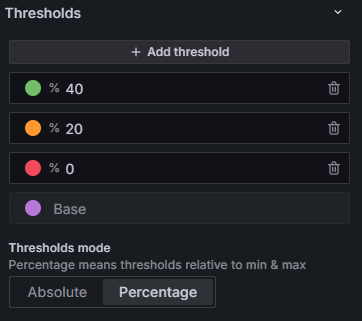
\includegraphics[width=0.6\textwidth, keepaspectratio]{images/thresholds.png}
    \caption{Grenzwerte für den \glqq Anteil der wiederkehrenden Besucher\grqq{}}
    \label{fig:thresholds}
\end{figure}

In Abbildung~\ref{fig:thresholds} ist zu erkennen, dass, wenn der Wert kleiner als 20 \% ist, die Farbe auf rot gesetzt wird. Zwischen 20 \% und 39 \% wird der Wert orange und ab 40 grün. Da es sich bei diesem Analysewert um ein Verhältnis handelt, muss der \texttt{Thresholds mode} entsprechend gesetzt werden, damit die Farben korrekt zugeordnet werden können. Damit diese Thresholds als Markierung an dem Panel angezeigt werden, wird zusätzlich die Option \texttt{Show threshold markers} aktiviert. Die Berechnung des Prozentwertes ist in Listing~\ref{lst:wiederkehrende-besucher} aufgezeigt:

\begin{figure}[H]
    \centering
    \begin{minipage}{\textwidth}
        \lstinputlisting[
            caption=Berechnung für den \glqq Anteil der wiederkehrenden Besucher\grqq{} in SQL,
            label={lst:wiederkehrende-besucher},
            language=sql
        ]{listings/wiederkehrende-besucher.sql}
    \end{minipage}
\end{figure}

Der Dividend entspricht der Anzahl der wiederkehrenden Besucher, während der Divisor die Gesamtzahl aller Besuche darstellt.

\subsection{Gerätetypen}
Für die Aufteilung der Gerätetypen wird, ebenfalls wie für die \glqq Verteilung der Traffic Quellen\grqq{}, ein Pie-Chart-Panel verwendet und in den Panel-Einstellungen genauso konfiguriert, um für ein konsistentes Design zu sorgen. Der einzige Unterschied ist, dass die Legende für diese Metrik aus Platzgründen rechts von dem Kreisdiagramm angezeigt wird.

\begin{figure}[H]
    \centering
    \begin{minipage}{\textwidth}
        \lstinputlisting[
            caption=Unterscheidung von Gerätetypen in Matomo,
            label={lst:geraetetypen},
            language=sql
        ]{listings/geraetetypen.sql}
    \end{minipage}
\end{figure}

Der Ausschnitt der Query für die Zuordnung (engl. Mapping) der Werte für die Gerätetypen ist in Listing~\ref{lst:geraetetypen} aufgelistet. Der \texttt{config\textunderscore device\textunderscore type} wird ebenfalls wie der \texttt{referer\textunderscore type} als Zahlenwert in der Datenbank gespeichert \parencite{GithubDevices}. Für den Fall, dass ein Gerät verwendet wird, welches nicht explizit gemappt wurde, wird der Wert \glqq Unknown\grqq{} gesetzt. Der \texttt{config\textunderscore device\textunderscore type} ist ebenfalls in der Tabelle \texttt{log\textunderscore visit} zu finden. 

\subsection{Bounce-Rate}
Die \glqq Bounce-Rate\grqq{} wird in Prozent angegeben und beschreibt, wie viele Nutzer nur eine einzige Aktion auf der Website durchgeführt haben und diese anschließend direkt wieder verlassen haben \parencite[S.33]{Dykes2014}. Da es sich bei dieser Metrik um ein Verhältnis handelt, wäre hierfür ein Gaug-Panel eine gute Wahl. Um das Dashboard jedoch übersichtlich zu halten und den Nutzer nicht mit zu vielen Gauge-Visualisierungen zu überfordern, wird die Bounce-Rate stattdessen in einem Stat-Panel dargestellt. Der Hintergrund wird hierbei, ebenso wie bei den bereits erläuterten Stat-Panels auf den Gelbton des Bildungsportals gesetzt.

Für die Berechnung wird das Attribut \texttt{visit\textunderscore total\textunderscore actions} der Tabelle \texttt{log\textunderscore visit} verwendet. Der Dividend bildet sich aus allen \texttt{visit\textunderscore total\textunderscore actions}, welche den Wert \glqq 1\grqq{} haben. Also aus allen Besuchen, in welchen nur eine Aktion erfolgt ist. Der Divisor ist die Anzahl aller Sitzungen.

\subsection{Verweildauer}
Für die Darstellung der Verweildauer wird ebenfalls ein Stat-Panel konfiguriert, da hierbei ein einzelner Zahlenwert zusammen mit der Einheit Minuten dargestellt wird. Auch hier wird der Gelbton des Bildungsportals als Hintergrundfarbe gesetzt.

Für diesen Analysewert kommen zwei Abfragen zum Einsatz, je nach Auswahl des Wertes für die Variable \texttt{\$Seite}. Für den Fall, dass \glqq Übersicht\grqq{} gewählt wurde, kann das Attribut \texttt{visit\textunderscore total\textunderscore time} aus der Tabelle \texttt{log\textunderscore visit} verwendet werden. Dieses Attribut gibt die Gesamtdauer einer Session an. In Listing~\ref{lst:duration-general} wird gezeigt, wie das Attribut verwendet wird, um die durchschnittliche Verweildauer für die gesamte Website zu bestimmen: 

\begin{figure}[H]
    \centering
    \begin{minipage}{\textwidth}
        \lstinputlisting[
            caption=Berechnung der durchschnittlichen Verweildauer auf dem Bildungsportal,
            label={lst:duration-general},
            language=sql
        ]{listings/duration-general.sql}
    \end{minipage}
\end{figure}

Hier wird zunächst die Dauer jeder einzelnen Session summiert und durch die gesammte Anzahl an Sitzungen, mittels \texttt{COUNT(*)} geteilt. \texttt{COUNT(*)} kann verwendet werden, da alle Spalten der \texttt{log\textunderscore visit}-Tabelle abgefragt werden. Daraufhin wird das Ergebnis durch 60 geteilt, um den Wert in Minuten zu erhalten. Schlussendlich wird das Ergebnis noch auf zwei Kommastellen abgerundet. 

Die Berechnung der Verweildauer auf einzelnen Unterseiten erfolgt auf eine andere Art und Weise. In Listing~\ref{lst:duration-sites} ist zu sehen, wie sich diese hierbei ergibt:

\begin{figure}[H]
    \centering
    \begin{minipage}{\textwidth}
        \lstinputlisting[
            caption=Berechnung der durchschnittlichen Verweildauer auf einer Unterseite des Bildungsportals,
            label={lst:duration-sites},
            language=sql
        ]{listings/duration-sites.sql}
    \end{minipage}
\end{figure}

Die Abfrage aus Listing~\ref{lst:duration-sites} berechnet die durchschnittliche Verweildauer der Nutzer auf einer bestimmten Seite oder auf allen Tagebuchseiten. Als Grundlage dafür wird eine verschachtelte SQL-Abfrage verwendet. Bei dieser werden zunächst für jeden Seitenaufruf die \texttt{start\textunderscore time} und \texttt{end\textunderscore time} ermittelt. Die \texttt{start\textunderscore time} wird von Matomo selbst gespeichert und stellt den Startzeitpunkt für den aktuellen Page-View dar. Die \texttt{end\textunderscore time} ist der Zeitpunkt des darauffolgenden Seitenaufrufs innerhalb der selben Session. Diese Endzeit wird durch eine Unterabfrage bestimmt, die innerhalb der selben Sitzung nach dem frühesten folgenden Seitenaufruf sucht. Hierfür wird \texttt{MIN(lva2.server\textunderscore time)} verwendet, wobei nur spätere Aktionen mit \texttt{type = 1}, also keine Events, berücksichtigt werden. Dadurch, dass die \texttt{SELECT}-Abfragen innerhalb von \texttt{FROM} erfolgen, wird eine temporäre Tabelle mit den beiden Spalten für die Start- und Endzeit erstellt. Mittels \texttt{TIMESTAMPDIFF()} wird abschließend die Differenz zwischen allen Start- und Endzeiten aus der Tabelle bestimmt und per \texttt{AVG()} wird der Durchschnitt gebildet. Das Ergebnis wird ebenfalls in Minuten umgewandelt und auf zwei Nachkommastellen begrenzt.

\subsection{KPIs}
Für alle vier KPIs wird ein Gauge-Panel erstellt. Die KPIs \glqq min. eine Tagebuchseite geöffnet\grqq{} und \glqq min. eine Überschrift aufgeklappt\grqq{} erhalten die Thresholds aus Listing~\ref{fig:thresholds-min-eins}. Die KPIs \glqq min. drei Tagebuchseiten geöffnet\grqq{} und \glqq min. drei Überschriften aufgeklappt\grqq{} bekommen die Thresholds aus Listing~\ref{fig:thresholds-min-drei}: 

\begin{figure}[H]
    \centering
    \begin{minipage}{0.49\textwidth}
        \centering
        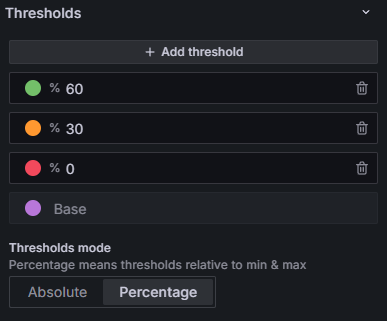
\includegraphics[width=\linewidth, keepaspectratio]{images/thresholds-min-eins.png}
        \caption{Grenzwerte für die KPIs \glqq min. eine Tagebuchseite geöffnet\grqq{} und \glqq min. eine Überschrift aufgeklappt\grqq{}}
        \label{fig:thresholds-min-eins}
    \end{minipage}
    \hfill
    \begin{minipage}{0.49\textwidth}
        \centering
        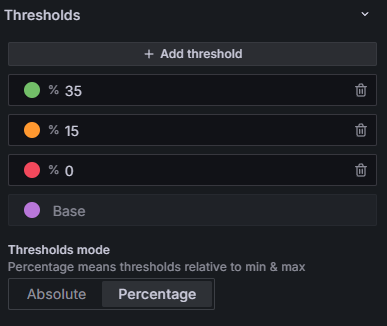
\includegraphics[width=\linewidth, keepaspectratio]{images/thresholds-min-drei.png}
        \caption{Grenzwerte für die KPIs \glqq min. drei Tagebuchseiten geöffnet\grqq{} und \glqq min. drei Überschriften aufgeklappt\grqq{}}
        \label{fig:thresholds-min-drei}
    \end{minipage}
\end{figure}

Die unterschiedlichen Thresholds verdeutlichen, dass für die beiden Arten von KPIs unterschiedliche Maßstäbe für den Erfolg gelten, da die Wahrscheinlichkeit, dass Nutzer eine Aktion dreimal ausführen, geringer ist als bei einer einmaligen Ausführung.

Die KPIs zu den Überschriften verwenden das in Listing~\ref{lst:headingsevent} gezeigte \texttt{expand}-Event. Die Tabellen \texttt{log\textunderscore visit} und \texttt{log\textunderscore link\textunderscore visit\textunderscore action} werden hierbei ebenso verknpüft, um die Events mit dem Namen \texttt{expand} zu filtern.
Dazu wird in einer Unterquery eine temporäre Tabelle gebildet, welche alle Sessions, in welchen eine Überschrift aufgeklappt wurde enthält. Diese Tabelle erhält den temporären Namen \texttt{visit\textunderscore with\textunderscore expand}. Der Divisor für das Verhältnis ist die Anzahl aller Sessions, also die Anzahl der Visit-ID's aus der Tabelle \texttt{log\textunderscore visit}. Da durch die Verwendung eines \texttt{LEFT JOIN} theoretisch mehrere Zeilen mit derselben \texttt{idvisit} entstehen können, wird in der Berechnung ein \texttt{DISTINCT} verwendet, um jede Sitzung nur einmal zu zählen. Somit ergibt sich die in Listing~\ref{lst:conversion-heading} zu sehende Berechnung für die Conversion-Rate für das Aufklappen der Überschriften: 

\begin{figure}[H]
    \centering
    \begin{minipage}{\textwidth}
        \lstinputlisting[
            caption=Berechnung der Conversion-Rate für \glqq min. eine Überschrift aufgeklappt\grqq{},
            label={lst:conversion-heading},
            language=sql
        ]{listings/conversion-heading.sql}
    \end{minipage}
\end{figure}

Der Ausdruck \texttt{visit\textunderscore all} ist hierbei ebenfalls wie \texttt{visit\textunderscore with\textunderscore expand} ein Alias für die Tabelle \texttt{log\textunderscore visit}. Für die Conversion \glqq min. drei Überschriften aufgeklappt\grqq{} wird zusätzlich über ein \texttt{HAVING} gefiltert, ob mindestens drei verschiedene Überschriften in einer Session aufgeklappt wurden. Die Berechnung der Conversion-Rate bleibt ansonsten gleich.

Für die KPI \glqq min. eine Tagebuchseite geöffnet\grqq{} wird berechnet, in wie vielen viele Sitzungen mindestens eine Tagebuchseite aufgerufen wurde. Da es sich bei jeder Tagebuchseite um eine eigene Unterseite handelt, ist für diese Metrik kein separates Event notwendig und es kann direkt über den Seitentitel gefiltert werden. Die Filterung erfolgt über den regulären Ausdruck \texttt{REGEXP 'Blatt [0-9]{4}'}. Das funktioniert, da die Titel für die Tagebuchseiten immer den Ausdruck \glqq Blatt XXXX\grqq{} enhalten, wobei jedes \glqq X\grqq{} für eine beliebige Zahlenkombination von null bis neun steht. Auch hier wird eine temporäre Tabelle gebildet, welche alle Visit-ID's der Sessions enthält, in welchen mindestens eine Tagebuchseite geöffnet wurde. Die Berechnung der Conversion-Rate erfolgt auf die gleiche Art und Weise wie in Listing~\ref{lst:conversion-heading}, nur das für den Dividenden die Menge der Einträge aus der temporären Tabelle summiert und verwendet werden. Für die KPI \glqq min. drei Tagebuchseiten geöffnet\grqq{} wird die gleiche Query wie für \glqq min. eine Tagebuchseite geöffnet\grqq{} verwendet. Zusätzlich wird über eine \texttt{HAVING}-Klausel gefiltert, dass nur Sitzungen gezählt werden, in denen mindestens drei verschiedene Tagebuchseiten aufgerufen wurden.

\subsection{Analyse einer Nutzersitzung}
Damit Nutzersitzungen individuell analysiert werden können, wird in den Grafana Einstellungen eine Query-Variable mit dem Namen \texttt{\$Session} erstellt. Die Query für die Variable gibt alle Sessions zurück, in welchen mindestens zwei Aktionen durch den Nutzer auf dem Bildungsportal erfolgt sind. Der Anwender kann die Visit-ID einer Session auswählen, welche daraufhin in der Abfrage zur Analyse der Nutzersitzung eingebunden wird. Außerdem werden die Visit-ID's in der Drop-Down Auswahl absteigend sortiert, sodass die aktuellste Session ganz oben angezeigt wird. Als Visualisierung für die Daten wird ein Gantt-Panel in Grafana verwendet, welches über ein Plugin eingebunden wird. Damit die Verweildauer des Besuchers korrekt auf der X-Achse dargestellt wird, wird die Option \texttt{Relativ time} ausgewählt. Somit wird die Zeit in Sekunden, bzw. Minuten angezeigt und nicht die Uhrzeit. Eine weitere Option mit dem Namen \texttt{Lock to extents} wird außerdem aktiviert. Das hat den Grund, da ansonsten der im Time Picker eingestellt Zeitraum für die Zeitbegrenzung auf der X-Achse verwendet wird. Über \texttt{Lock to extents} wird sichergestellt, dass die frühste Startzeit und die aktuellste Endzeit einer Sitzung für die Begrenzung der X-Achse gesetzt wird. Auf der Y-Achse werden die Titel der aufgerufenen Seiten sowie die Namen der ausgelösten Events in der Session angezeigt. Für die Balken, welche die Länge eines Page-Views und die Länge eines Events darstellen, wird ein Color-Mapping verwendet. Hierbei erhalten die Events die gleiche Farbe wie die Seite, auf welcher sie ausgelöst wurden. Somit kann über den Namen an der X-Achse und auch über die Farbe direkt erkannt werden, zu welcher Unterseite ein Event gehört. Alle Tagebuchseiten, werden in der Farbe grün dargestellt, sowie auch die dazugehörigen Überschriften-Events. Ebenfalls werden Unterseiten, welche zum Reiter \glqq Wer war Eva Schiffmann?\grqq{} gehören auch in einer einheitlichen Farbe dargestellt, damit keine verschiedenen Farbtöne einer Farbe genutzt werden müssen. Auch für die Events, welche auf Unterseiten von \glqq Wer war Eva Schiffmann?\grqq{} ausgelöst werden wird ein einheitlicher Farbton gesetzt. Unterseiten des Reiters \glqq Themen\grqq{} sowie Events auf diesen Unterseiten erhalten gleichermaßen einen einheitlichen Farbton. Da Events und Page-Views auf einer Seite den selben Farbton verwenden, wird zusätzlich ein Label für die Aktionen gesetzt, welches angibt, ob es sich um einen Page-View, ein Audio-Event, ein Video-Event, einen Outlink oder um ein Überschriften-Event handelt. Outlinks sind die in der Website eingebetteten Links, welche auf externe Websiten verweisen.

Um die korrekte Endzeit für ein Überschriften-Event zu setzen, wird das in Listing~\ref{lst:headingsevent} dargestellte \texttt{close}-Event und der enthaltene Zeitstempel genutzt. Um zu erfassen, wann ein Nutzer ein Video abspielt und wann dieser das Abspielen beendet, werden die in Listing~\ref{lst:video-event} dargestellten Events definiert: 

\begin{figure}[H]
    \centering
    \begin{minipage}{\textwidth}
        \lstinputlisting[
            caption=Matomo-Events für die Erfassung der Abgespielten Videos,
            label={lst:video-event},
        ]{listings/video-events.js}
    \end{minipage}
\end{figure}

Die in den Zeilen 6 und 16 verwendete Variable \texttt{videoTitle} wird über einen Query-Selector ermittelt, welcher das abgepsielte Video im Programmcode selektiert. Anschließend wird das \texttt{<h3>}-Element, welches den Titel des Videos beinhaltet extrahiert und als \texttt{videoTitle} gesetzt. Audio-Events funktionieren auf die gleiche Art und Weise, erhalten aber als Kategorie den Wert \texttt{audio} und als Label den \texttt{audioTitle}, welcher ebenso ermittelt wird wie der \texttt{videoTitle}.

Da innerhalb einer Sitzung unterschiedliche Arten von Nutzerinteraktionen auftreten können, umfasst die Abfrage insgesamt fünf Unterqueries. Jeweils eine für Page-Views, Audio-, Video- und Outlink-Interaktionen sowie Überschriften-Events. Diese Unterqueries werden über ein \texttt{Union} miteinander kombiniert. Das Ergebnis dieses \texttt{Union} ist eine Liste von allen Aktionen, welche innerhalb der Session durchgeführt wurden und bildet somit die Gesamtmenge der Ergebnisse der Unterqueries. Diese Ergebnismenge wird schlussendlich nach der Startzeit der Aktionen sortiert. Somit kann der zeitliche Verlauf korrekt im Gantt-Panel angezeigt werden. Die Unterqueries sind so strukturiert, dass diese alle die gleichen Attribute erzeugen. Diese Attribute sind der Titel, die Startzeit, die Endzeit und die Kategorie, welche für das Label an den Balken verwendet wird. Um die Endzeit korrekt zu berechnen, wird die gleiche Logik wie in Listing~\ref{lst:duration-general} angewendet. Hierbei wird wieder ermittelt, welches das frühste \texttt{close}-Event, für ein vorheriges \texttt{open}-Event ist. Es muss darauf geachtet werden, dass eine Endzeit nur gesetzt wird, wenn die Kategorie des \texttt{close}-Events die gleiche ist wie bei dem \texttt{open}-Event. Ansonsten würde nach jeder Aktion die Endzeit für die vorherige Aktion gesetzt werden. Das hätte zur Folge, dass \texttt{close}-Events ebenfalls die Endzeit für Page-Views setzen würden. Um die Endzeit eines Page-Views zu ermitteln, greift die gleiche Logik wie bei den Events. Nur das diese nicht per Event bestimmt wird, sondern dem Zeitstempel des nachfolgenden Seitenaufrufs entspricht. Für die letzte Unterquery, welche die Outlinks betrifft, wird eine feste Verweildauer von einer Sekunde verwendet. Da nicht getrackt werden kann, wie viel Zeit ein Nutzer auf der externen Website verbringt. Outlinks werden von Matomo selbst in der Tabelle \texttt{log\textunderscore link\textunderscore visit\textunderscore action} gespeichert, in welcher sich ebenfalls alle Page-Views befinden. Damit nur tatsächliche Outlinks erfasst werden und nicht alle Page-Views, erhält die Unterquery noch die Bedinung \texttt{NOT LIKE 'localhost/evaschiffmann\%'}.

\section{Die Dashboards im Überblick}
Das erstellte Gantt-Diagramm ist in der Abbilung~\ref{fig:gantt-diagramm} zu erkennen:

\begin{figure}[H]
    \centering
    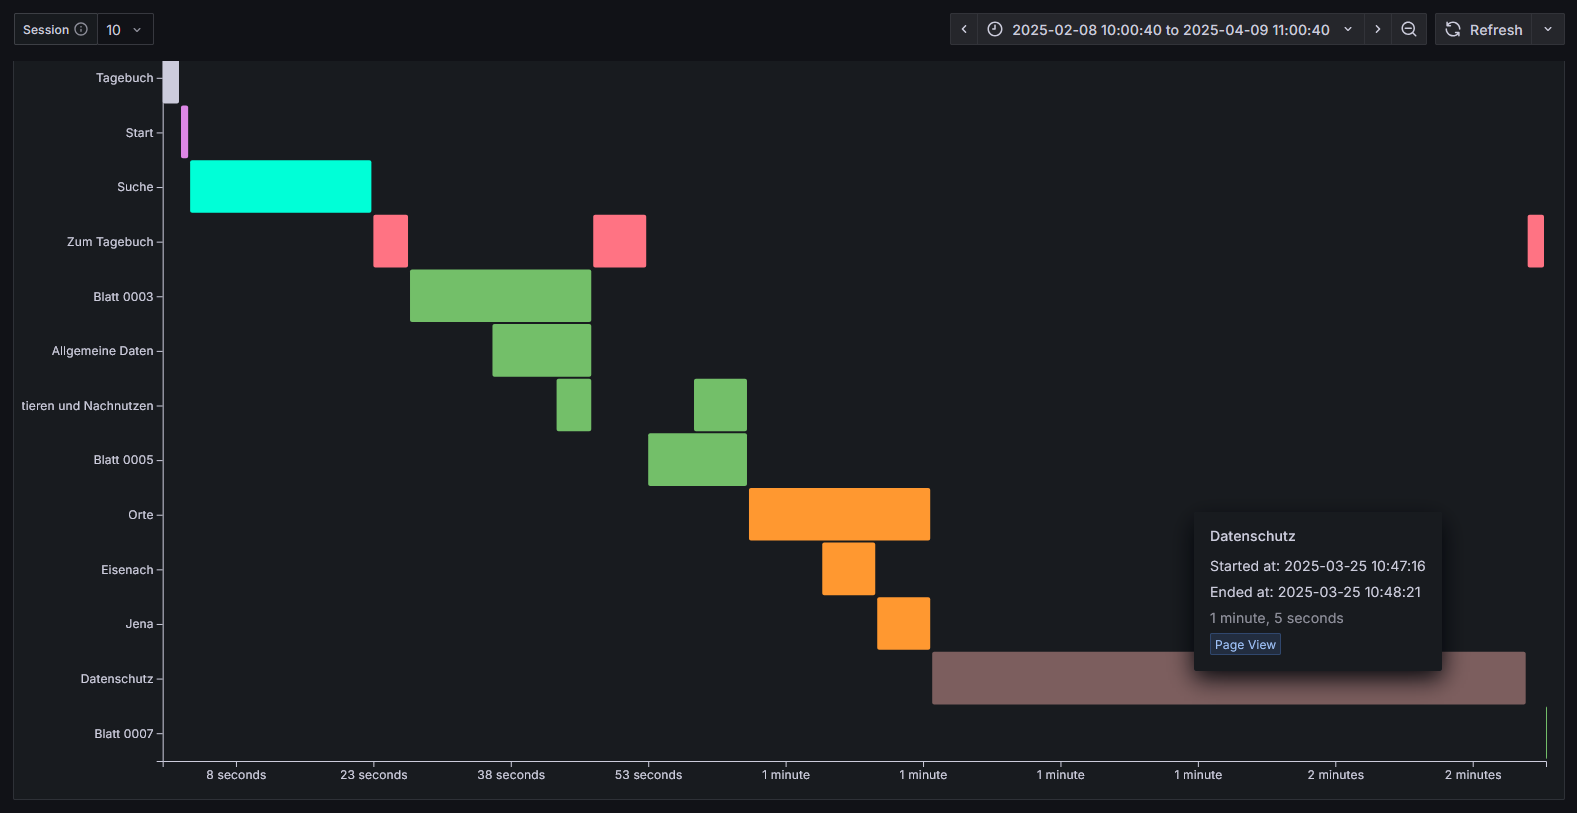
\includegraphics[width=1\textwidth, keepaspectratio]{images/nutzerpfade.png}
    \caption{Gantt-Diagramm zur Analyse einzelner Nutzersitzungen}
    \label{fig:gantt-diagramm}
\end{figure}

Oben links in der Abbildung kann die präferierte Session ausgewählt werden. Die auf der Abbildung dargestellte Session weist eine Verweildauer von etwas mehr als zwei Minuten auf und es wurden sowohl Page-Views als auch Events ausgelöst. Ebenfalls ist zu erkennen, dass beim Überfahren der Balken mit der Maus ein Pop-up erscheint, welches den Nutzer über die Verweildauer sowie über die Art der Aktion informiert.

In der Abbildung~\ref{fig:haupt-dashboard} ist das erstellte Haupt-Dashboard mit den einzelnen Analysewerten aufgeführt:

\begin{figure}[H]
    \centering
    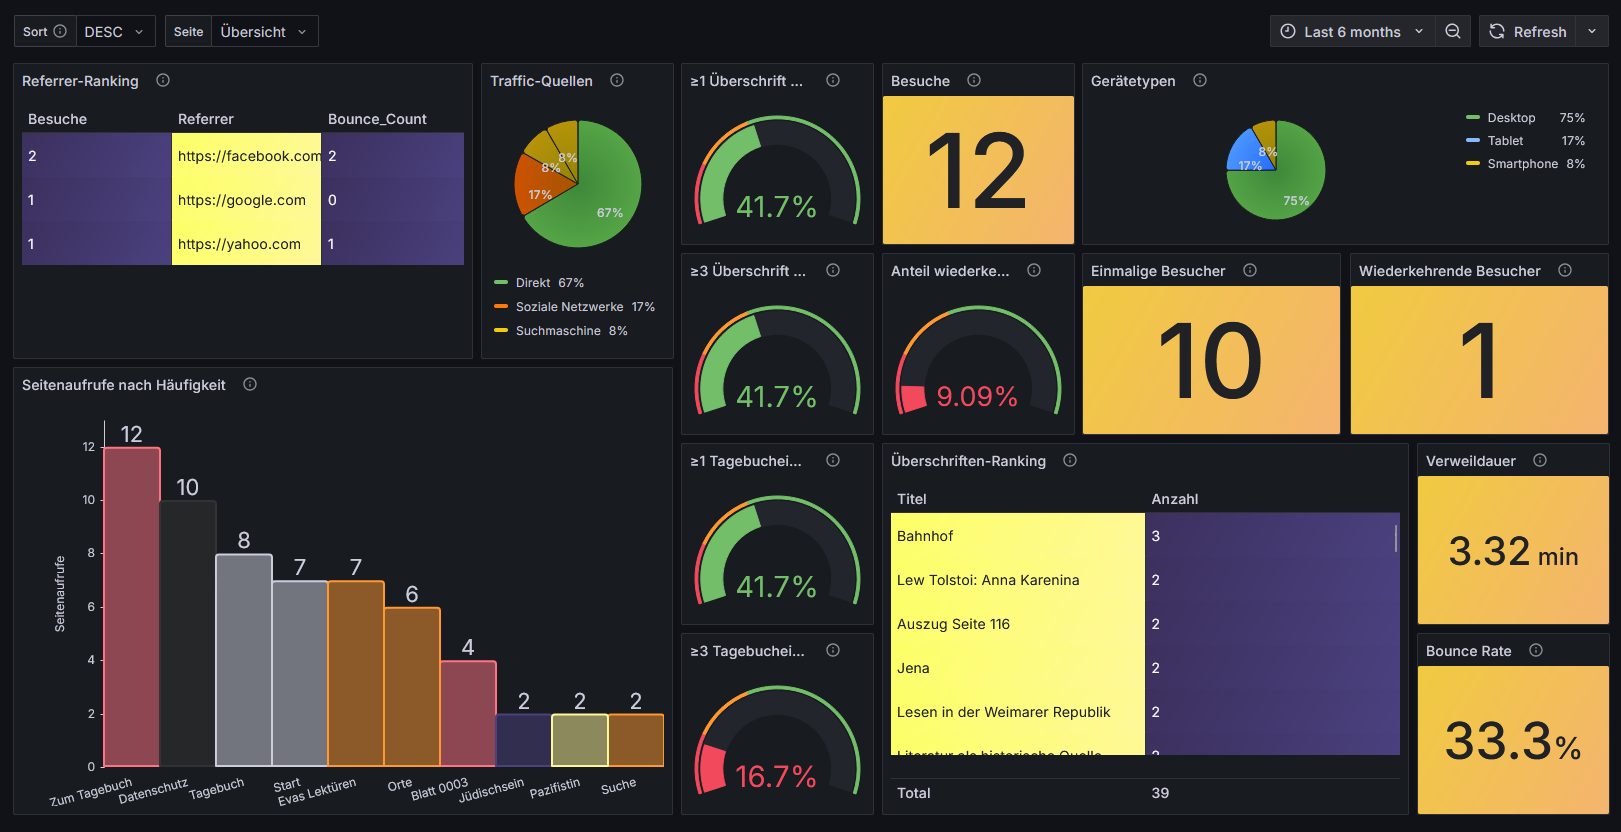
\includegraphics[width=1\textwidth, keepaspectratio]{images/fertiges-dashboard.png}
    \caption{Haupt-Dashboard, zur Visualisierung der Analysewerte}
    \label{fig:haupt-dashboard}
\end{figure}

Am oberen linken Rand des Dashboards werden die Variablen \texttt{\$Sort} und \texttt{\$Seite} angezeigt. Am oberen rechten Rand des Dashboards kann der Zeitbereich über den Time Picker ausgewählt werden. Mit dem Refresh-Button lassen sich alle SQL-Abfragen aktualisieren, sodass die neuesten Daten im Dashboard angezeigt werden. Die Analysewerte wurden entsprechend den jeweiligen Dimensionen angeordnet. Eine Ausnahme bildet die Metrik \glqq Ranking der am häufigsten aufgeklappten Überschriften\grqq{}. Diese wurde aus Platzgründen unten rechts in der Dimension \glqq Verhalten\grqq{} platziert, obwohl diese inhaltlich der Dimension \glqq Inhalte\grqq{} zuzuordnen ist. Da allerdings die beiden Metriken für die Dimension \glqq Inhalte\grqq{} viel Platz erfordern und eine kleinere Darstellung der Panels die Übersichtlichkeit negativ beeinflussen würde, wurde die Metrik daher bewusst an alternativer Stelle positioniert.
    \chapter{Evaluation}
\label{ch:evaluation}

\section{Technische Evaluation}
\label{sec:technische-evaluation}
Ziel der technischen Evaluation ist es, zu überprüfen, ob die im Konzept definierten Anforderungen erfolgreich umgesetzt wurden.

\textbf{Datenintegration und Aggregation}

Die Datenintegration zwischen Matomo und Grafana wurde erfolgreich über eine direkte MySQL-Datenquelle in Grafana realisiert. Da Grafana nur lesenden Zugriff auf die Matomo-Datenbank hat, wird sichergestellt, dass die Rohdaten nicht verändert werden können. Die Daten können mithilfe von SQL-Abfragen aggregiert und im Dashboard als Analysewerte dargestellt werden. Außerdem können in Grafana alle SQL-Abfragen über einen Refresh-Button ausgeführt werden, wodurch direkt die aktuellsten Daten zur Verfügung stehen. An diesem Button kann ebenfalls ein Intervall für die Aktualisierung eingestellt werden. Dadurch kann die Aktualisierung der Analysedaten in definierten Intervallen erfolgen. Somit ist diese Anforderung erfüllt.

\textbf{Sicherheit und Zugriffskontrolle}

Matomo und Grafana sind durch die Verwendung eines Revers Proxy unter einer einheitlichen Domain und ausschließlich über HTTPS verfügbar. Ebenso verfügen beide Tools über eine RBAC, sodass nur Administratoren Änderungen vornehmen können, während reguläre Nutzer ausschließlich Leseberechtigungen für die Tools erhalten. Dadurch wird unberechtigter Zugriff verhindert und die Anforderung ist erfüllt. 

\textbf{Transparenz}

Auf der Datenschutzseite der Website war bereits ein umfassender Hinweistext vorhanden. Damit wird die Transparenz gewährleistet. In diesem Hinweistext wird der Nutzer über die Erhebung und Verwendung der durch Matomo erfassten Daten sowie den Einsatz von Cookies zu Analysezwecken informiert. Dies deutet darauf hin, dass Matomo bereits zuvor zur Webanalyse auf dem Bildungsportal eingesetzt wurde. 

\textbf{Datenminimierung}

Es werden ausschließlich anonyme Nutzerdaten erfasst, welche für die Verhaltensanalyse benötigt werden, womit das Prinzip der Datenminimierung eingehalten wird. Ebenfalls werden keine personenbezogenen Daten gesammelt und der Nutzer wird ausschließlich über eine ID identifiziert. Wenn der Nutzer den Tracking-Cookie löscht, kann dieser auch nicht mehr der ID zugeordnet werden und er erhält eine neue ID, falls der Cookie später erneut akzeptiert wird.

\textbf{Einwilligung}

Das Tracking erfolgt ausschließlich nach ausdrücklicher Zustimmung durch den Nutzer. Dies wurde durch ein Opt-In über das bestehende Cookie-Consent-Banner realisiert. Zusätzlich wurde ein Opt-Out über die Datenschutzseite implementiert, mit dem die Einwilligung jederzeit widerrufen werden kann und der Tracking-Cookie gelöscht wird. Somit werden die Vorgaben der DSGVO eingehalten und die Anforderung ist erfüllt.

Da alle Anforderung vollständig umgesetzt wurden, wird die technische Evaluation als erfolgreich bewertet. Die entwickelte Lösung erfüllt die datenschutzrechtlichen Vorgaben und ermöglicht ebenfalls die Echtzeitübertragung der Daten an das Dashboard-Tool. 

\section{Nutzerevaluation}
\label{sec:nutzer-evaluation}
Die Evaluation des Dashboards wurde anhand einer Nutzerbefragung in Form eines Fragebogens durchgeführt. Dieser umfasst insgesamt 34 Fragen und enthält sowohl offene als auch geschlossene Antwortmöglichkeiten. Einige Fragen mussten nicht zwingend beantwortet werden. Diese sollten nur dann ausgefüllt werden, wenn konkrete Verbesserungswünsche zu einem bestimmten Aspekt bestehen oder eine Antwort näher begründet werden sollte. Alle Fragen und Antworten sind im Anhang aufgeführt. Der Fragebogen gliedert sich in drei Abschnitte, welche im Folgenden separat ausgewertet werden.

\textbf{Allgemeine Einschätzung des Dashboards}

Das Dashboard wurde insgesamt positiv bewertet. Die Übersichtlichkeit und die Nutzerfreundlichkeit wurden mit vier von fünf Sternen bewertet. Laut Herrn Staack stellen die beiden Dashboards eine geeignete Grundlage zur Analyse des Nutzerverhaltens auf dem Bildungsportal dar, da sie sowohl statistische Auswertungen als auch die Nachverfolgung einzelner Sitzungsverläufe ermöglichen. Kritisch angemerkt wurde, dass einzelne Tagebuchseiten nicht separat ausgewertet werden können. Die Interaktionsdaten für diese werden aktuell über die Auswahl \glqq Alle Tagebuchseiten\grqq{} zusammengefasst. Eine Möglichkeit zur Einzelanalyse der unterschiedlichen Tagebuchseiten wäre jedoch zusätzlich wünschenswert. Die Interaktivitätsfunktionen, also die Auswahl eines bestimmten Zeitraums, die Möglichkeit zur Analyse einzelner Unterseiten sowie die Sortierung der Rankings wurden durchweg als sehr hilfreich bewertet. Auch die Beschriftungen der Panels und der Beschreibungstext wurden als gut verständlich eingestuft. Die Farbgestaltung des Dashboards wird als intuitiv empfunden und erleichtert die Analyse. Obwohl das Dashboard als übersichtlich eingestuft wurde, könnten laut Herrn Staack die Panels zur Bounce-Rate und zu den Gerätetypen anders angeordnet werden, sodass auf der rechten Seite des Dashboards alle Analysewerte angezeigt werden, welche sich über die Variable \texttt{\$Seite} filtern lassen. Ebenfalls ist noch ein weiteres Event wünschenswert, welches die Interaktionen mit den Bildern auf dem Bildungsportal erfasst. 

\textbf{Analyse einzelner Nutzersitzungen}

Die entwickelte Lösung zur Nachvollziehbarkeit von Nutzersitzungen im Gantt-Diagramm wurde von Herrn Staack mit fünf von fünf Sternen bewertet. Die Visualisierung wird als verständlich empfunden und ermöglicht eine detaillierte Analyse der Nutzerinteraktionen. Auch die farbliche Unterscheidung der Aktionen sowie die ergänzenden Beschriftungen an den Balken, die die Art der Aktion und deren Dauer anzeigen, wurden als sinnvoll und hilfreich beurteilt. In diesem Bereich wurden keine Verbesserungsvorschläge geäußert. Insgesamt bieten die dargestellten Interaktionen nach Einschätzung von Herrn Staack eine gute Grundlage zur Analyse von Sitzungsverläufen. Lediglich die ergänzende Darstellung von Bildinteraktionen im Diagramm wird als wünschenswert genannt.

\textbf{Metriken und KPIs}

Laut Herrn Staack decken die vorhandenen Analysewerte die relevanten Anforderungen an die Analyse des Nutzerverhaltens auf dem Bildungsportal ab. Es wurde kein Analysewert genannt, welcher als überflüssig oder wenig hilfreich empfunden wurde. Die Bewertungen aller Metriken in den Bereichen Besucher, Inhalte, Verhalten sowie Traffic-Quellen fielen mit jeweils fünf von fünf Sternen sehr positiv aus. Auch die Darstellung der Konversionen wird als zielgerichtet und sinnvoll wahrgenommen. Die Visualisierungen der Analysewerte wurden insgesamt als gut verständlich beurteilt. Der einzige Verbesserungsvorschlag ist auch hier eine zusätzliches Event für die Interaktion mit den Bildern auf dem Bildungsportal.

Die über den Fragebogen identifizierten Verbesserungspotenziale konnten aus zeitlichen Gründen nicht mehr im Rahmen dieser Arbeit umgesetzt werden. Ursache hierfür war die verspätete Bereitstellung der Datenbasis, wodurch der Entwicklungsprozess zeitlich eingeschränkt wurde. Die erfassten Änderungswünsche bilden jedoch eine fundierte Grundlage für weiterführende Anpassungen des Dashboards, die über den zeitlichen Rahmen dieser Arbeit hinaus umgesetzt werden können. Zudem ist hervorzuheben, dass die einzelnen Panels per Drag-and-Drop neu angeordnet werden können, wodurch Nutzer das Layout individuell und nach eigenen Präferenzen anpassen können.
    %! suppress = UnresolvedReference


\chapter{Persönliche Reflexion, Fazit und Ausblick}
\label{ch:zusammenfassung}

\section{Persönliche Reflexion}
Die Umsetzung dieser Bachelorarbeit war sowohl fachlich als auch organisatorisch herausfordernd. Da das ursprünglich vorgesehene TYPO3-Projekt, das als Grundlage für die Analyse des Bildungsportals dienen sollte, nicht rechtzeitig zur Verfügung stand, konnte der geplante Meilensteinplan nicht wie vorgesehen eingehalten werden. Um diese Situation zu überbrücken, wurde zunächst mit den theoretischen Kapiteln begonnen und eine konzeptionelle Ausarbeitung der Lösung vorgenommen. Gleichzeitig wurden die Tools zunächst in eine im Laufe des Studiums erstellte Website integriert, um trotzdem Erfahrungen für die Implementierung und Konfiguration zu sammeln. Eine weitere Herausforderung war die vollständige Einrichtung der Container-Umgebung. Ebenso bestanden zu Beginn der Arbeit keine Vorkenntnisse in der Konfiguration und dem Aufsetzen von Webservern, weshalb sich dieses Wissen im Verlauf der Arbeit zusätzlich angeeignet werden musste. Anfangs waren die Dienste lediglich über Angabe separate Ports für die Dienste in der URL erreichbar. Erst durch weitere Recherche konnte eine Lösung mit einem Reverse Proxy umgesetzt werden. Über diesen konnten alle Dienste unter einer gemeinsamen Domain und individuellen Pfaden zugänglich gemacht werden, wodurch die Integration in die Live-Umgebung später erleichtert wird. Auch die Integration der Matomo-Daten in Grafana stellte zunächst eine Herausforderung dar. Die ursprüngliche Idee, hierfür die Reporting-API von Matomo zu verwenden, erwies sich als zu unflexibel, da die benötigten Informationen nicht in dem Detail gefiltert werden konnten, wie es für die Analysewerte erforderlich war. Insbesondere im Bezug auf die selbstdefinierten Grafana-Variablen. Um die Metriken und KPIs in der gewünschten Detailtiefe und Aktualität zu erfassen, war es erforderlich, spezifische SQL-Abfragen auf die Datenbank von Matomo anzuwenden. 

Trotz oder auch gerade wegen diesen Hürden wurde im Verlauf der Arbeit sehr viel neues Wissen erlangt und bestehendes Wissen vertieft. Es wurde keine vorgefertigte Lösung übernommen, sondern auf Grundlage eigener Anforderungen und intensiver Recherche eine individuelle Lösung für das Bildungsportal entwickelt. Dabei konnte nicht nur fundiertes Wissen im Bereich der Webanalyse und datenschutzkonformen Datenverarbeitung aufgebaut werden, sondern auch die praktische Umsetzung eines Dashboards realisiert werden. Zudem wurden bestehende Kenntnisse in SQL, JavaScript, Python und Docker-Compose erweitert und gefestigt.

Insgesamt konnte ich durch diese Arbeit wertvolle Erfahrungen in der Softwareentwicklung und insbesondere im Bereich der Webanalyse und Datenvisualisierung sammeln – sowohl technisch als auch konzeptionell. 

\section{Fazit}
Ziel dieser Arbeit war die Entwicklung eines Web-basierten Analysetools für das Bildungsportal \textit{evaschiffmann.de}, das eine datenschutzkonforme Erhebung sowie eine effektive und aussagekräftige Visualisierung von Nutzerdaten ermöglicht. Im Rahmen der Implementierung wurde ein vollständiges Tracking- und Visualisierungssystem konzipiert und implementiert, das auf den Open-Source-Tools Matomo und Grafana basiert.

Die im Konzept definierten Anforderungen an Datenschutz, Datenintegration, Aggregation sowie Sicherheit und Zugriffskontrolle, welche in den Kapiteln~\ref{ch:webanalyse} und~\ref{ch:auswahl} motiviert wurden, konnten erfolgreich umgesetzt werden. Dies wurde im Rahmen der technischen Evaluation aufgezeigt. Auch die Nutzerevaluation durch Herrn Staack zeigt, dass die entwickelte Lösung den gewünschten Anforderungen in hohem Maße gerecht wird. Die grafischen Darstellungen, Filterfunktionen und Visualisierungen wurden insgesamt als hilfreich, verständlich und benutzerfreundlich empfunden. Besonders die Analyse einzelner Nutzersitzungen im Gantt-Diagramm und die Sinnhaftigkeit der ausgewählten Analysewerte wurde hierbei sehr positiv bewertet. Die Verbesserungspotenziale, also die Ergänzung eines Events zur Erfassung von Bildinteraktionen und die Möglichkeit zur separaten Auswertung einzelner Tagebuchseiten, konnten aus zeitlichen Gründen nicht mehr vollständig umgesetzt werden. Diese Aspekte wurden in der Evaluation klar benannt und können als Grundlage für eine mögliche letzte Optimierung verwendet werden.

Die Arbeit zeigt insgesamt, dass es möglich ist, kostenlos und mit frei verfügbaren Tools eine datenschutzkonforme und dennoch aussagekräftige Webanalyse zu realisieren. Die entwickelte Lösung kann im Live-Betrieb dazu beitragen, besser zu verstehen, wie Nutzer mit dem digitalisierten historischen Wissen auf dem Bildungsportal umgehen. Darüber hinaus kann die Lösung dafür verwendet werden, eventuelle Verbesserungspotentiale der Website zu identifizieren.

Die zentrale Forschungsfrage für die Arbeit lautete: 

\textit{„Wie kann ein Web-basiertes Analysetool für das Bildungsportal \textit{evaschiffmann.de} entwickelt werden, das eine datenschutzkonforme Erhebung und eine effektive Visualisierung von Nutzerdaten für eine aussagekräftige Analyse ermöglicht?“}

Die durchgeführte Implementierung und die Evaluation zeigen auf, wie eine solche Lösung konkret realisiert werden kann, wodurch die Forschungsfrage beantwortet ist. Die entwickelte Anwendung erfüllt die datenschutzrechtlichen Vorgaben, ermöglicht eine strukturierte Analyse der erhobenen Daten und unterstützt durch die grafische Aufbereitung im Dashboard effektiv die Auswertung des Nutzerverhaltens. Damit wurde das Ziel dieser Arbeit erreicht.

\section{Ausblick}
Die entwickelte Lösung zur Analyse des Nutzerverhaltens ist nicht ausschließlich auf das Bildungsportal \textit{evaschiffmann.de} beschränkt, sondern lässt sich grundsätzlich auch auf andere Bildungsportale und Websites übertragen. Insbesondere die im Dashboard enthaltene Darstellung einzelner Nutzersitzungen in Form eines Gantt-Diagramms bietet eine flexible und visuell anschauliche Möglichkeit, Nutzerinteraktionen zeitlich geordnet abzubilden. Durch eine entsprechende Anpassung der erfassten Events kann dieses Diagramm auch Seitenwechsel, Interaktionen innerhalb von Seiten sowie das Verlassen der Seite über externe Links auf anderen Webseiten abbilden.

Für zukünftige Arbeiten ergeben sich verschiedene Forschungsansätze. Denkbar wäre etwa, alternative Formen zur Visualisierung einzelner Nutzersitzungen zu erproben, um komplexe Interaktionsverläufe noch anschaulicher darzustellen. Ebenso könnten Verfahren zur automatisierten Erkennung typischer Nutzungspfade mithilfe KI-gestützter Analysemodelle entwickelt werden. Solche Verfahren könnten dabei helfen, das Verhalten auf Bildungsplattformen nicht nur schneller, sondern auch präziser auszuwerten. Gerade im Kontext digitaler Lernangebote eröffnen sich dadurch neue Wege, um das Nutzerverhalten besser zu verstehen. 



   
% --- Ab hier in Römischen Zahlen nummerieren
    \pagenumbering{Roman}
    \setcounter{page}{\value{exterior}}

%--------------------------------------
%   Literaturverzeichnis mit BibLaTeX
%--------------------------------------
%%--------------------------------------
%%   BibLateX - Literaturverzeichnis
%%--------------------------------------

    \printbibliography
    \cite{Eurostat}
    \cite{Potomac}
    \cite{Alby2019}
    \cite{Hassler2019}
    \cite{Dykes2014}
    \cite{Apache}
    \cite{Hanschke2020}
    \cite{DSGVO}
    \cite{Voigt2020}
%--------------------------------------
%   Glossar
%--------------------------------------
    %\printglossaries

%--------------------------------------
%   Selbstständigkeitserklärung und Anhang
%--------------------------------------
    \addchap{Selbstständigkeitserklärung}
Ich, \autor, versichere hiermit, dass ich die vorliegende \art  { }mit dem Thema

\begin{quote}
    \textit{\titel} \textit{\untertitel}
\end{quote}

selbstständig und nur unter Verwendung der angegebenen Quellen und Hilfsmittel angefertigt habe.

\begin{flushright}
    \ort, \datum
\end{flushright}
\small{\autor} 
    \addcontentsline{toc}{chapter}{\appendixname}
\appendix


%\chapter{Skripte}
%\label{ch:skripte}
%	\lstinputlisting[caption={Converterprogramm von alten zu neuen Konfigurationsdateien},label=app:conv]{Quellen/env2imp.java}
%	\lstinputlisting[language=ANT,caption={Angepastes Ant-Buildskript},label=app:antinstall]{Quellen/build.xml}
%	\lstinputlisting[caption={Batchdatei zum Automatischen Verteilen},language=command.com,label=app:batchjenkins]{Quellen/depoly_DMSCore.bat}


%\chapter{Konfigurationen}
%\label{ch:konfigurationen}
%	\lstinputlisting[caption={Alte Konfiguration},label=konf:oldkonf]{Quellen/Environment.properties}
%	\lstinputlisting[caption={Importdatei mit den Werten der alten Konfigurationsdatei},language=XML,label=konf:xmlfuerdms]{Quellen/out.xml}

\chapter{Ausgefüllter Fragebogen}
\label{app:fragebogen}

Im Folgenden ist der von Herrn Staack ausgefüllte Fragebogen zur Bewertung des Dashboards vollständig aufgeführt.

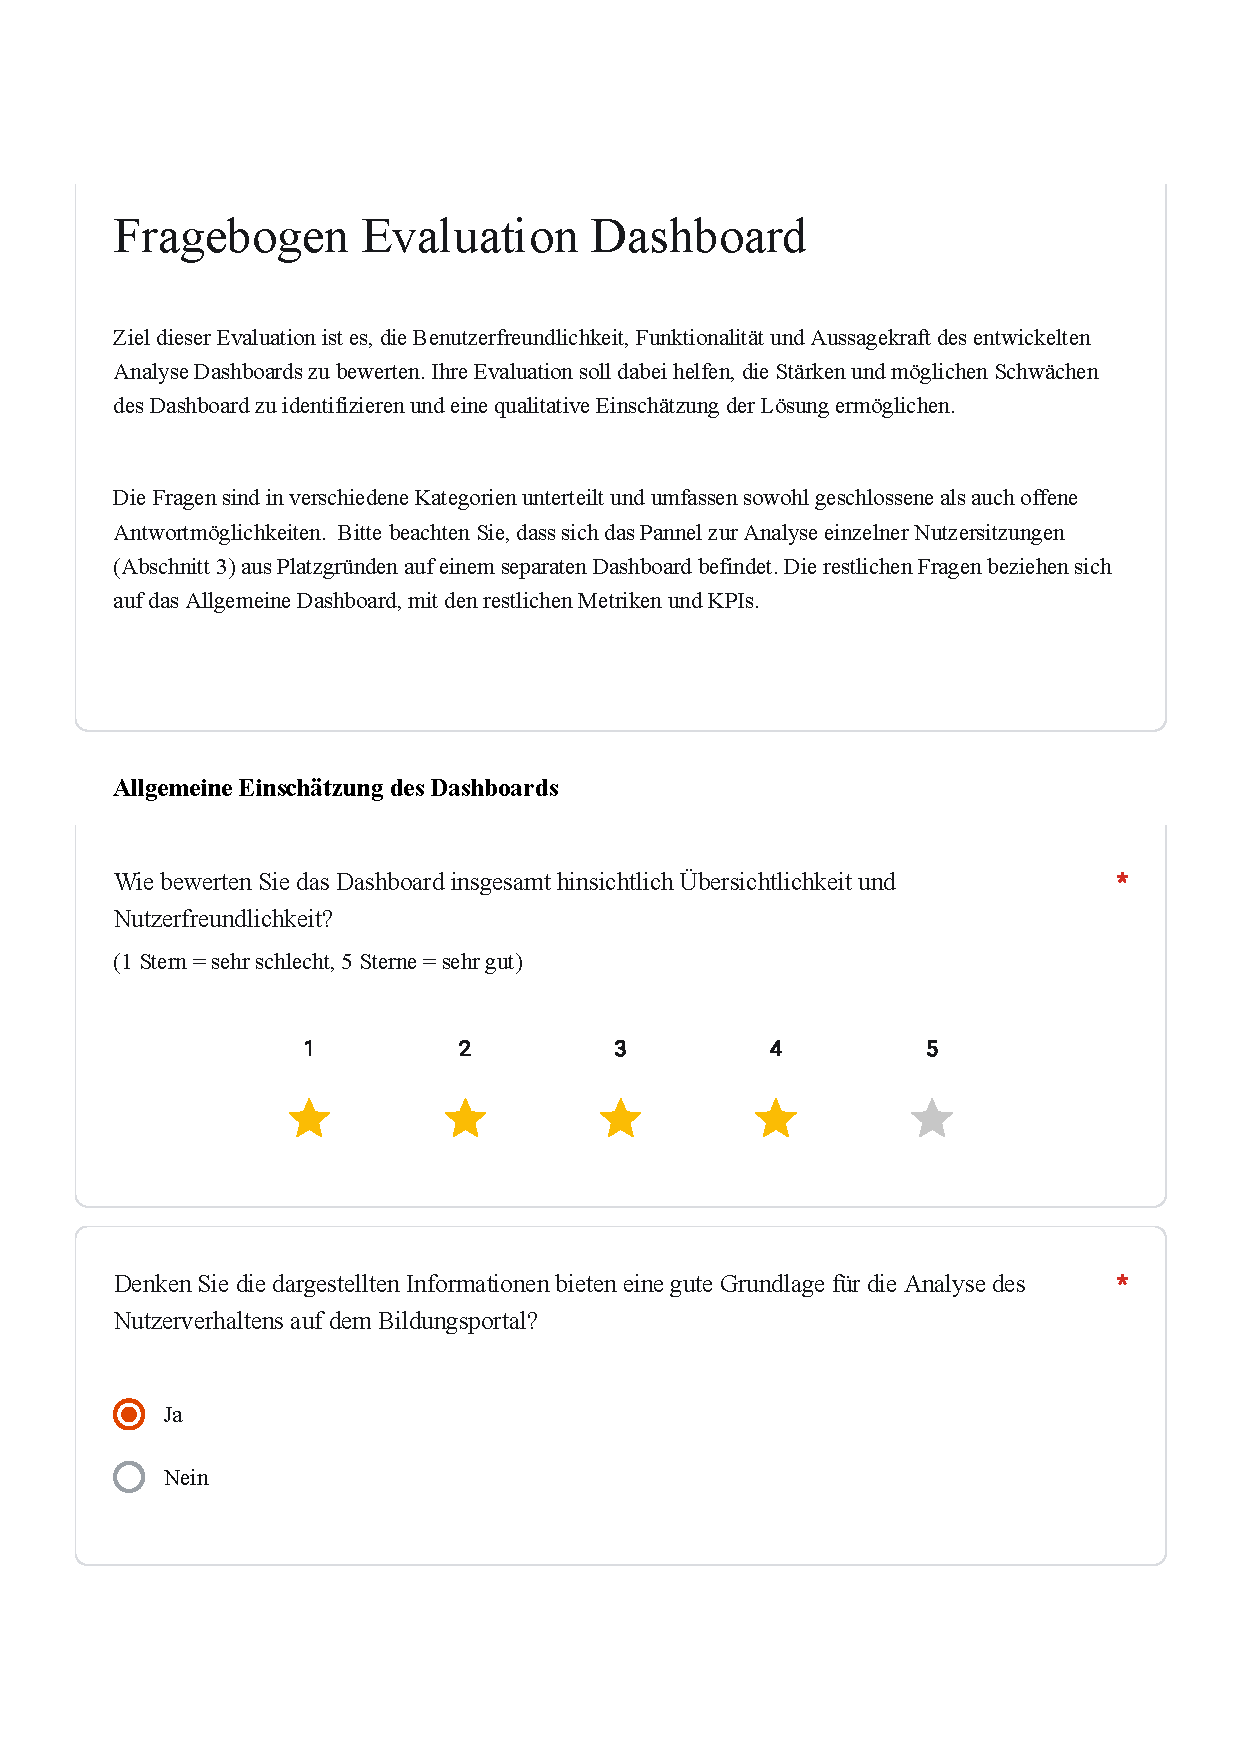
\includepdf[
  pages=-,
  pagecommand={},
  trim=1cm 1cm 1cm 1cm,
  clip,
  width=\textwidth
]{images/fragebogen-ausgefuellt.pdf}

\clearpage

\end{document}